\documentclass[a4paper,10pt]{article}
\usepackage{tabularx} % extra features for tabular environment
\usepackage{amsmath,amssymb,amsfonts,amsthm}  % improve math presentation
\usepackage{graphicx} % takes care of graphic including machinery
\usepackage{geometry} % decreases margins
\geometry{
  a4paper,
  right=20mm,
  left=20mm,
  top=20mm,
}

%HEADER
%\usepackage{fancyhdr}
%\pagestyle{fancy}
%\lhead{This is my name}
%\rhead{this is page \thepage}
% chktex-file 44
% chktex-file 3
% chktex-file 1
% chktex-file 12
% chktex-file 24
% chktex-file 46
% chktex-file 8
% chktex-file 36

%REFS, CITATI
\usepackage[final]{hyperref} % advs hyper links inside the generated pdf file

\usepackage[backend=biber, style=numeric, sorting=none]{biblatex}
\addbibresource{ref.bib} % <-- Add your .bib file name here

\hypersetup{
	colorlinks=true,       % false: boxed links; true: colored links
	linkcolor=blue,        % color of internal links
	citecolor=blue,        % color of links to bibliography
	filecolor=magenta,     % color of file links
	urlcolor=blue         
}
\renewcommand{\figurename}{Slika}
\renewcommand{\tablename}{Tabela}

%PACKIGI
\usepackage{physics}
\usepackage{mathtools}
\usepackage{bm}
\usepackage{placeins}
\usepackage{tcolorbox}
\usepackage{lipsum}
\usepackage{gensymb}
\usepackage{siunitx}
\usepackage{mdframed}
\usepackage{empheq}
\usepackage{caption}
\usepackage{subcaption}
\usepackage{enumitem}
\usepackage{icomma}
\usepackage{colortbl}
\usepackage{multirow}
\usepackage{dsfont}
\usepackage{fontspec}
\usepackage[version=4]{mhchem}
\usepackage{cuted} 
\usepackage{algorithm}
\usepackage{booktabs}
\usepackage{algpseudocode}
\usepackage{scalerel}
\usepackage{simpler-wick}
\newcommand\Dag{\scalerel*{\dag}{X}}
% ---------------------------------------------------------------
\algnewcommand\algorithmicreturnx{\textbf{return}}
\algnewcommand\Ret{\State \algorithmicreturnx{} }
 

%tikz
\usepackage{tikz}
\usepackage[compat=1.1.8]{tikz-feynman}
%jeziki
\usepackage[slovene]{babel}

%FONT SETUP
\setmainfont{Libertinus Serif}

\setsansfont{Schnebel Sans Pro}[
  BoldFont = {Schnebel Sans Pro Bold},
  UprightFont = {Calibri}]

%CAPTION SETUP
\usepackage[labelfont=bf, font={sf, footnotesize}, labelformat=simple]{caption}
\DeclareCaptionFormat{nature}{\textbf{#1#2}~\footnotesize#3}
\DeclareCaptionLabelSeparator{pipe}{\,$\bm{|}$}

\captionsetup
{
    format=nature,
    labelsep=pipe
}

%SECTION/SUBSECTION SETUP
\usepackage[sc]{titlesec}
% \titleformat*{\section}{\Large\scshape\bfseries\centering}
% \titleformat*{\subsection}{\large\scshape\bfseries\centering}
% \titleformat*{\subsubsection}{\subsubsectionfont\centering}
\titleformat*{\section}{\Large\bfseries\sffamily\centering}
\titleformat*{\subsection}{\large\bfseries\sffamily\centering}
\titleformat*{\subsubsection}{\normalsize\bfseries\sffamily\centering}


%MISC
\usepackage{xprintlen}
\DeclareMathOperator\arctanh{arctanh}

\definecolor{titlegray}{gray}{0.9}
\definecolor{lightgray}{gray}{0.92} 

\renewcommand{\vec}[1]{\mathbf{#1}}
\AtBeginDocument{\RenewCommandCopy\qty\SI}

\newcommand{\dg}[5]{%
  \begin{tikzpicture}[baseline=(v),x=10mm,y=10mm]
    \begin{feynman}
      \vertex (q) at (-1.6,0);
      \vertex (v) at (0,0);
      \vertex (u) at (0.8,1);
      \vertex (l) at (0.8,-1);
      \diagram*{
        (l) -- [fermion] (v) -- [fermion] (u),
        #1
      };
    \end{feynman}
    \node[below] at (-0.9,-0.15) {$#2$};
    \node[right] at (u) {$#3$};
    \node[right] at (l) {$#4$};
    \node[right] at (v) {$#5$};
  \end{tikzpicture}%
}

%________________________________________________________________________________
\begin{document}
% \begin{titlepage}
% \scshape

% \centering
% 
\includegraphics[width=12cm, keepaspectratio]{UL_FMF-logoENG-HOR-CMYK_color.pdf} \par \vspace{0.5cm}



% \raisebox{-\baselineskip}{\rule{\textwidth}{1pt}}
% \rule{\textwidth}{1pt}
% \vspace{0.2cm}

%     {\fontsize{24pt}{26pt}\selectfont\bfseries Teorija trdne snovi} \par \vspace{0.1cm}
% {\fontsize{14pt}{20pt}\selectfont Peierlsova nestabilnost}

% \raisebox{-\baselineskip}{\rule{\textwidth}{1pt}}
% \rule{\textwidth}{1pt}
% \vspace{0.2cm}
% \vspace{1cm}


% {\fontsize{12pt}{18pt}\selectfont
% Korl Železnikar\\ \vspace{0.2cm}
% Mentorja: doc. dr. Denis Golež}

% \vspace{2cm}




% \vfill
% {\fontsize{12pt}{18pt}\selectfont \today}

% \end{titlepage}

\section{Osnove teorije}
\subsection{BCS teorija pri končni temperaturi}
BCS model, kjer je $\xi_{\vec{k}, \sigma} = \epsilon_{\vec{k}, \sigma} - E_F$ in $k := (\vec{k}, \uparrow)$, $-k := (\vec{-k}, \downarrow)$:
\begin{align}
  H = \sum_k \xi_k (c_k^\dagger c_k + c_{-k}^\dagger c_{-k}) - V \sum_{k,k'} c_k^\dagger c_{-k}^\dagger c_{-k'} c_{k'}
\end{align}
Naredimo približek povprečnega polja, definiramo $b_k = c_{k} c_{-k}$ in $b_k = \langle b_k\rangle + \delta b_k = F_k  + \delta b_k$, sledi (do $\mathcal{O}(\delta b_k^2)$)
\begin{align}
  b_k^\dagger b_{k'} \simeq  F_k^* F_{k'} + F_k^* \delta b_{k'} + F_{k'} \delta b_k^\dagger = F_k^* b_{k'} + F_{k'} b_k^\dagger - F_k^* F_{k'} =  \langle b_k^\dagger \rangle b_{k'} + b_k^\dagger \langle b_{k'} \rangle - \langle b_k^\dagger \rangle \langle b_{k'} \rangle 
\end{align}
Iz česar sledi: 
\begin{align}
  H = \sum_k \begin{pmatrix} c_k^\dagger & c_{-k} \end{pmatrix} \begin{pmatrix} \xi_k & -\Delta_k \\ -\Delta_k^* & -\xi_k \end{pmatrix} \begin{pmatrix} c_k \\ c_{-k}^\dagger \end{pmatrix} + \frac{\vert{}\Delta\vert{}^2}{V} + \sum_k \xi_k
\end{align}
Ob definiciji $\Delta_k = \sum_{k'} V(k-k') \langle c_{k'}c_{-k'}\rangle$, vzamemo še lokalno interakcijo, zato je $V(q)\simeq V$ in $\Delta_k \simeq \Delta$. Naredimo Bogoljubov rotacijo, privzamemo $u_k, v_k \in \mathbb{R}$ in simetrijo okoli $E_F$: $u_k = u_{-k}$ ter $v_k = v_{-k}$. Iz  CCR sledi $u_k^2+v_k^2=1$. 
Kvazidelci so definirani z rotacijo 
\begin{align}
  \begin{pmatrix} c_k \\ c_{-k}^\dagger \end{pmatrix} = \begin{pmatrix} u_k & v_k \\ -v_k & u_k \end{pmatrix} \begin{pmatrix} \alpha_k \\ \alpha_{-k}^\dagger \end{pmatrix}
\end{align}
nov Hamiltonjan pa postane
\begin{align}
  H = \sum_k \begin{pmatrix} \alpha_k^\dagger & \alpha_{-k} \end{pmatrix}   \begin{pmatrix} \xi_k u_k^2 + u_k v_k (\Delta_k + \Delta_k^*) - \xi_k v_k^2 & -2\xi_k u_k v_k + \Delta_k u_k^2 - \Delta_k^* v_k^2 \\ -2\xi_k u_k v_k - \Delta_k v_k^2 + \Delta_k^* u_k^2 & \xi_k v_k^2 - \xi_k u_k^2 + u_k v_k (\Delta_k + \Delta_k^*) \end{pmatrix} \begin{pmatrix} \alpha_k \\ \alpha_{-k}^\dagger \end{pmatrix}\,,
\end{align} 
kjer zahtevamo, da so izvendiagonalni členi enaki 0. Iz CCR zahteve lahko vzamemo parameterizacijo (tu sem vzel kompleksno nastavimo, da je $\Delta = \Delta^* e^{i2\phi_k}$):
\begin{align}
v_k &= \sin\left(\frac{\theta_k}{2}\right) e^{i\phi_k} \\
u_k &= \cos\left(\frac{\theta_k}{2}\right) \\
u_k v_k &= \cos\left(\frac{\theta_k}{2}\right) \sin\left(\frac{\theta_k}{2}\right) = \frac{1}{2} \sin\theta_k\\
u_k^2 - v_k^2 &= \cos^2\left(\frac{\theta_k}{2}\right) - \sin^2\left(\frac{\theta_k}{2}\right) = \cos\theta_k 
\end{align}
skupaj dobimo (od tu naprej $\Delta := |\Delta|$): 
\begin{align}
  \xi_k \sin(\theta_k) =  \Delta \cos(\theta_k)
\end{align}
kar fiksira 
\begin{align}
  \tan(\theta_k) = \frac{|\Delta_k|}{\xi_k}\,.
\end{align}
Tako iz trikotnika preberemo
\begin{align}
  \sin\theta_k = \frac{\vert{}\Delta_k\vert{}}{E_k} = \frac{\vert{}\Delta_k\vert{}}{\sqrt{\xi_k^2 + \vert{}\Delta_k\vert{}^2}} \\
  \cos\theta_k = \frac{\xi_k}{E_k} = \frac{\xi_k}{\sqrt{\xi_k^2 + \vert{}\Delta_k\vert{}^2}} \\
\end{align}
kjer je $E_k = \pm\sqrt{\xi_k^2 + \vert{}\Delta_k\vert{}^2}$ energija kvazidelcev:
\begin{align}
  H = \sum_k E_k \alpha_k^\dagger \alpha_k - E_k \alpha_{-k}^\dagger \alpha_{-k} + \xi_k +  \frac{|\Delta|^2}{V}\,.
\end{align} 
V termičnem stanju so diagonalni delci porazdeljeni po 
\begin{align}
  \langle \alpha_k^\dagger \alpha_k\rangle = \frac{1}{1+ \exp(E_k / T)} = \frac{1}{2}-\frac{1}{2} \tanh\left(\frac{E_k}{2T}\right)\,.
\end{align}
Uporabni sta zvezi $f(-E/T) = 1-f(E/T)$ in $1-2f(E/T) = \tanh(E/(2T))$. V definiciji ureditvenega parametra je 
\begin{align}
  \langle c_k c_{-k} \rangle = \left\langle \left( u_k \alpha_k - v_k \alpha_{-k}^\dagger \right) \left( u_k \alpha_{-k} + v_k \alpha_k^\dagger \right) \right\rangle= u_k v_k \left( 1 - \langle \alpha_{-k}^\dagger \alpha_{-k} \rangle - \langle \alpha_k^\dagger \alpha_k \rangle \right) = \frac{1}{2} \sin\theta_k \tanh\left(\frac{\beta E_k}{2}\right)
\end{align}
iz česar sledi enačba za režo pri $T>0$ (seštevamo po $k$ okoli $E_F$):
\begin{align}
  \Delta = \frac{V}{2} \sum^{'}_k \sin\theta_k \tanh\left(\frac{E_k}{2T}\right) = \frac{V \Delta}{2} \sum_k \frac{\tanh\left(\frac{1}{2T} \sqrt{\Delta^2 + \xi_k^2}\right)}{\sqrt{\Delta^2 + \xi_k^2}}
\end{align}
\subsection{Minimalni model ekscitonskega izolatorja pri končni temperaturi}
Pri izolatorju za minimalni model vzamemo dve orbitali ($a, b$) model tesne vezi v vsaki posebej in lokalno Coulombovo interakcijo na mestu $j$ med elektronskima gostotama v posameznih pasovih 
\begin{align}
  H = H_0 + H_V &= \sum_{i,j} \left( \epsilon_a^{(0)} \delta_{ij} + t_{ij}^{(a)} \right) c_{a,i}^\dagger c_{a,j} + \sum_{i,j} \left( \epsilon_b^{(0)} \delta_{ij} + t_{ij}^{(b)} \right) c_{b,i}^\dagger c_{b,j} + V \sum_j c_{a,j}^\dagger c_{a,j} c_{b,j}^\dagger c_{b,j} \\
  &= \sum_k \varepsilon_{a,k} c_{a,k}^\dagger c_{a,k} + \sum_k \varepsilon_{b,k} c_{b,k}^\dagger c_{b,k} + V \sum_j c_{a,j}^\dagger c_{a,j} c_{b,j}^\dagger c_{b,j}
\end{align}
najprej diagonaliziramo vsako orbitalo posebej, kar da gole disperzije (vezavni energiji nastavimo na $\pm G/2$) (delamo v dveh dimenzijah in mrežna konstanta $a_0=1$): 
\begin{align} \label{free el tb}
  \varepsilon_{a(b),\vec k} = \pm \frac{G}{2} - 2 t_{a(b)}(\cos(k_x) + \cos(k_y))\,,
\end{align}
v tem primeru je najmanjša razdalja med pasovoma $G_0 = G - 4 (t_a -t_b)$ oziroma $G_0=G - 8t_a$, če je $t_b = -t_a$. Za interakcijo spet naredimo približek povprečnega polja: 
\begin{align}
  c_{a,j}^\dagger c_{a,j} c_{b,j}^\dagger c_{b,j} \approx \langle c_{a,j}^\dagger c_{a,j} \rangle c_{b,j}^\dagger c_{b,j} + \langle c_{b,j}^\dagger c_{b,j} \rangle c_{a,j}^\dagger c_{a,j} - \langle c_{a,j}^\dagger c_{b,j} \rangle c_{b,j}^\dagger c_{a,j} - \langle c_{b,j}^\dagger c_{a,j} \rangle c_{a,j}^\dagger c_{b,j} + \text{konst.}
\end{align}
od tod sledi
\begin{align}
  H_V^{\text{MF}} = V n_b \sum_j c_{a,j}^\dagger c_{a,j} + V n_a \sum_j c_{b,j}^\dagger c_{b,j} - V \phi \sum_j c_{b,j}^\dagger c_{a,j} - V \phi^* \sum_j c_{a,j}^\dagger c_{b,j} + N V \vert{}\phi\vert{}^2
\end{align}
kjer smo definirali: 
\begin{align}
  n_a = \langle c_{a,j}^\dagger c_{a,j} \rangle = \frac{1}{N} \sum_k \langle c_{a,k}^\dagger c_{a,k} \rangle
\end{align}
\begin{align}
  n_b = \langle c_{b,j}^\dagger c_{b,j} \rangle = \frac{1}{N} \sum_k \langle c_{b,k}^\dagger c_{b,k} \rangle
\end{align}
\begin{align}
  \phi = \langle c_{a,j}^\dagger c_{b,j} \rangle = \frac{1}{N} \sum_k \langle c_{a,k}^\dagger c_{b,k} \rangle \\
  \Delta = -\frac{V}{N} \sum_k \langle c_{a,k}^\dagger c_{b,k} \rangle, \quad \Delta^* = -\frac{V}{N} \sum_k \langle c_{b,k}^\dagger c_{a,k} \rangle
\end{align}
\begin{align}
  \Delta_k = \frac{1}{N} \sum_{k'} V(k - k') \langle a_{k'}^\dagger b_{k'} \rangle, \quad V(q) = \int e^{-i \vec{q} \cdot \vec{r}} V(\vec{r}) \, \dd{\vec{r}}
\end{align}
Uporabimo FT še na celotnem Hamiltonjanu
\begin{align}
  c_{a,j}^\dagger = \frac{1}{\sqrt{N}} \sum_k e^{-i \vec{k} \cdot \vec{r}_j} c_{a,k}^\dagger
\end{align}
\begin{align}
  H^{\text{MF}} = \sum_k \left( [\varepsilon_{a,k} + V n_b] c_{a,k}^\dagger c_{a,k} + [\varepsilon_{b,k} + V n_a] c_{b,k}^\dagger c_{b,k} + \Delta^* c_{a,k}^\dagger c_{b,k} + \Delta c_{b,k}^\dagger c_{a,k} \right) + \left( \frac{\vert{}\Delta\vert{}^2}{V} N - V N n_a n_b \right)
\end{align}
oziroma: 
\begin{align}
  H^{\text{MF}} = \sum_k \begin{pmatrix} c_{a,k}^\dagger & c_{b,k}^\dagger \end{pmatrix} \begin{pmatrix} {\varepsilon}^H_{a,k} & \Delta^* \\ \Delta & {\varepsilon}^H_{b,k} \end{pmatrix} \begin{pmatrix} c_{a,k} \\ c_{b,k} \end{pmatrix} + \text{konst.}\,,
\end{align}
kjer definiramo Hartree energiji ${\varepsilon}^H_{a(b),k} = \varepsilon_{a(b),k} + V n_{b(a)}$. Transformacija v diagonalno  / Bogoljubov bazo je podobna kot pri BCS, le da ne meša kreatorjev in anihilatorjev / ohranja število delcev:
\begin{align} \label{EI_uintana_rotacija}
  \begin{pmatrix} c_{a,k} \\ c_{b,k} \end{pmatrix} = \begin{pmatrix} u_k & v_k \\ -v_k & u_k \end{pmatrix} \begin{pmatrix} \alpha_k \\ \beta_k \end{pmatrix}
\end{align}
od tod po enakem postopku kot prej dobimo energiji kvazidelcev
\begin{align}
E_{\alpha(\beta)}(k) = \frac{{\varepsilon}^H_{a,k} + {\varepsilon}^H_{b,k}}{2} \pm \sqrt{\left(\frac{{\varepsilon}^H_{a,k} - {\varepsilon}^H_{b,k}}{2}\right)^2 + \vert{}\Delta\vert{}^2} := \eta_k \pm \sqrt{\xi_k^2 +\Delta^2}
\end{align}
Za bookkeeping: 
\begin{align}
  \left( \frac{\varepsilon_a^H - \varepsilon_b^H}{2} \right)& \sin \theta_k + \Delta \cos \theta_k = 0 \implies \tan \theta_k = \frac{-2 \Delta}{\varepsilon_a^H - \varepsilon_b^H} = \frac{-\Delta}{\xi_k}\\
  u_k v_k &= -\frac{\sin \theta_k}{2}\,.
\end{align}
Za samousklajeno enačbo zdaj potrebujemo
\begin{align}
  \langle c_{a,k}^\dagger c_{b,k} \rangle = \langle (u_k \alpha_k^\dagger + v_k \beta_k^\dagger)(-v_k \alpha_k + u_k \beta_k) \rangle = u_k v_k \left( \langle \beta_k^\dagger \beta_k \rangle - \langle \alpha_k^\dagger \alpha_k \rangle \right) = -\frac{1}{2} \sin\theta_k (f(E_{\beta}) - f(E_{\alpha}))
\end{align}
od tod
\begin{align}
  \Delta = -\frac{V}{N}\sum_k \langle c_{a,k}^\dagger c_{b,k} \rangle = \frac{V}{N} \sum_k \frac{ \Delta}{2\sqrt{\xi_k^2 + \vert{}\Delta\vert{}^2}} (f(E_{\beta}) - f(E_{\alpha}))
\end{align}
Opomba, lahko definiramo tudi $n = n_a + n_b = \text{konst.} = 1$ in $n_a-n_b =: m$ od tod sledi

\begin{align}
  H^{\text{MF}} = \sum_k \left( \left[\varepsilon_{a,k} + \frac{V}{2}n - \frac{V}{2}m\right] c_{a,k}^\dagger c_{a,k} + \left[\varepsilon_{b,k} + \frac{V}{2}n +\frac{V}{2}m\right] c_{b,k}^\dagger c_{b,k} + \Delta^* c_{a,k}^\dagger c_{b,k} + \Delta c_{b,k}^\dagger c_{a,k} \right)
\end{align}
od koder je v 2D Hartree gap enak: 
\begin{align}
  G^H = G-4(t_a-t_b) - V m\,. 
\end{align}
Note: v praksi je $m<0$
V dveh dimenzijah se Hartree pasova srečata na 
\begin{align}
  \mu_B = \frac{V}{2}n - \frac{t_a + t_b}{t_a-t_b}\frac{G-Vm}{2}\,.
\end{align}
Zamik je enak $V/2$, ko sta osnovna pasova simetrična in je zasedenost polovična. V primeru simetričnih pasov sta disperziji kvazidelcev
\begin{align}
  E_{\alpha(\beta)}(k) - V/2 = \pm \sqrt{\left(\frac{{\epsilon}_{a,k} - {\epsilon}_{b,k} - Vm}{2}\right)^2 + \vert{}\Delta\vert{}^2}\,.
\end{align}
Velja še
\begin{align}
  n_a &= \frac{1}{N} \sum_k \left( u_k^2 f(E_\alpha) + v_k^2 f(E_{\beta}) \right) \\
  n_b &= \frac{1}{N} \sum_k \left( v_k^2 f(E_\alpha) + u_k^2 f(E_{\beta}) \right)
\end{align}

\begin{align}
  u_k^2 &= \frac{1}{2}\left(1 + \frac{\xi_k}{\sqrt{\Delta^2 + \xi_k^2}}\right) \\
  v_k^2 &= \frac{1}{2}\left(1 - \frac{\xi_k}{\sqrt{\Delta^2 + \xi_k^2}}\right)
\end{align}
\begin{align}
  m = n_a-n_b = \frac{1}{N}\sum_{\vec{k}} \frac{\xi_\vec{k}}{\sqrt{\xi_\vec{k}^2+\Delta^2}} (f(E_\alpha) - f(E_{\beta}))
\end{align}
\subsection{Numerika/psevdokoda}

\subsection{Odprti sistemi in modeliranje kopeli}
Born-Markov master enačbe in Redfield: ločimo kopel in sistem, 
\begin{align}
  \rho_{S}(t) = \text{Tr}_{B}(\rho(t))
\end{align}
Hamiltonjan razcepimo na $H = H_0 + H_I$, kjer je $H_0 = H_S \otimes \mathbb{I}_B + \mathbb{I}_S \otimes H_B$ razdenjen na podsistema, za interakcijski del pa privzamemo obliko $H_I = \sum_\alpha A_\alpha \otimes B_\alpha$. V interakcijski sliki je operator za evolucijo
\begin{align}
  U_{0}(t, t_{0}) = e^{-i H_{0}(t - t_{0})}
\end{align}
\begin{align}
  \rho_I(t) &= U_0^\dagger(t, 0) \rho(t) U_0(t, 0) = e^{i H_0 t} \rho(t) e^{-i H_0 t}\\
  H_I(t) &= U_0^\dagger(t, 0) H_I U_0(t, 0) = e^{i H_0 t} H_I e^{-i H_0 t}
\end{align}
Von Neumannova enačba je 
\begin{align}
  \frac{d}{dt}\rho_I(t) &= -i [H_I(t), \rho_I(t)] \\
  \rho_I(t) &= \rho_I(0) - i \int_{0}^{t} dt' \, [H_I(t'), \rho_I(t')]
\end{align}
vstavimo nazaj v komutator in se znebimo prostosnih stopenj kopeli:
\begin{align} \label{VN-integrated}
  \frac{d}{dt}\rho_{S}(t) = -\int_{0}^{t} ds \, \text{Tr}_{B}\left( [H_{I}(t), [H_{I}(t-s), \rho_{S}(t) \otimes \rho_{B}]] \right)
\end{align}
V interakcijskem členu so operatorji $A_\alpha$ napisani kot lastni operatorji $H_S$ z energijami prehodov $\omega = E_b - E_a$
\begin{align}
  A_\alpha(\omega) = \sum_{E_b - E_a = \omega} \vert{}a\rangle \langle a\vert{} A_\alpha \vert{}b\rangle \langle b\vert{}
\end{align}
To zadošča relacijam $[H_S, A_\alpha(\omega)] = -\omega A_\alpha(\omega), \quad [H_S, A_\alpha^\dagger(\omega)] = \omega A_\alpha^\dagger(\omega)$ in \\ $e^{i H_S t} A_\alpha(\omega) e^{-i H_S t} = e^{-i \omega t} A_\alpha(\omega), \quad e^{i H_S t} A_\alpha^\dagger(\omega) e^{-i H_S t} = e^{i \omega t} A_\alpha^\dagger(\omega)$. V interakcijski sliki potem velja
\begin{align}
  H_I(t) = \sum_{\alpha, \omega} e^{-i \omega t} A_\alpha(\omega) \otimes B_\alpha(t) = e^{i H_B t} B_\alpha e^{-i H_B t} 
\end{align}
evolucija sledi kot
\begin{align}
  \dot{\rho}_{S} = \sum_{\omega, \omega'} \sum_{\alpha, \beta} e^{i(\omega' - \omega)t} \Gamma_{\alpha\beta}(\omega) \left( A_{\alpha}(\omega) \rho_{S}(t) A_{\beta}^{\dagger}(\omega') - A_{\beta}^{\dagger}(\omega') A_{\alpha}(\omega) \rho_{S}(t) \right) + \text{h.c.}
\end{align}
kjer so prehodne matrike med stanji
\begin{align}
  \Gamma_{\alpha\beta}(\omega) = \int_{0}^{\infty} ds \, e^{i\omega s} \, \text{Tr}_{B}\left( B_{\alpha}^{\dagger}(t) B_{\beta}(t-s) \rho_{B} \right) = \frac{1}{2}\gamma_{\alpha\beta}(\omega) + i S_{\alpha\beta}(\omega)
\end{align}
Evolucija pa ima strukturo
\begin{align}
  \frac{d\rho_{S}}{dt} = -i [H_{LS}, \rho_{S}(t)] + \mathcal{D}(\rho_{S}(t))
\end{align}
z disipatorjem
\begin{align}
  \mathcal{D}(\rho_{S}) = \sum_{\omega} \sum_{\alpha,\beta} \gamma_{\alpha\beta}(\omega) \left( A_{\beta}(\omega) \rho_{S} A_{\alpha}^{\dagger}(\omega) - \frac{1}{2} \{ A_{\alpha}^{\dagger}(\omega) A_{\beta}(\omega), \rho_{S} \} \right)
\end{align}
oz. v splošnem
\begin{align}
  \mathcal{D}(\rho_{S}) = \sum_{k} \gamma_{k} \left( L_{k} \rho_{S} L_{k}^{\dagger} - \frac{1}{2} \{ L_{k}^{\dagger} L_{k}, \rho_{S} \} \right)
\end{align}
V stacionarnem stanju velja
\begin{align}
  \mathcal{L}\rho_{\text{ness}} = 0\,.
\end{align}
Notes za vektorizacijo in superoperatorje: 
\begin{align}
\mathcal{L} u_{\mu}^R = \lambda_{\mu} u_{\mu}^R
\end{align}  
\begin{align}
  \text{vec}(ABC) = (A \otimes C^T) \text{vec}(B)
\end{align}
\begin{align}
  \text{Tr}(A^{\dagger} B) = \text{vec}(A)^{\dagger} \text{vec}(B)
\end{align}
\begin{align}
  \frac{d}{dt}\vert{}\rho\rangle = \left( -i H \otimes \mathbb{I} + i \mathbb{I} \otimes H^T + \sum_{k} L_{k} \otimes L_{k}^* - \frac{1}{2} \sum_{k} (L_{k}^{\dagger} L_{k} \otimes \mathbb{I} + \mathbb{I} \otimes L_{k}^T L_{k}^*) \right) \vert{}\rho\rangle
\end{align}
\begin{align}
  \langle \hat{O} \rangle(t) = \langle \mathbb{I} \vert{} \hat{O} \otimes \mathbb{I} \vert{} \rho(t) \rangle
\end{align}
Šibke sklopitve in perturbacijski pristopi
\begin{align}
  \mathcal{L} = -i [H, \cdot] + \epsilon \mathcal{D}[\cdot], \quad  \quad \rho = \rho_{0} + \epsilon \rho_{1} + \epsilon^2 \rho_{2} + \dots
\end{align}
napišemo gostotno matriko sistema v lastni bazi, siagonalno, s klasičnimi populacijami
\begin{align}
  \rho_{0} = \sum_{n} p_{n} \vert{}n\rangle \langle n\vert{}, \quad H\vert{}n\rangle = E_{n} \vert{}n\rangle
\end{align}
kjer velja v ničtem redu (by construction)
\begin{align}
  \mathcal{L}\rho_0 = -i [H, \rho_0] = 0
\end{align}
V prvem redu so enačbe za NESS
\begin{align}
  -i [H, \rho_1] + \mathcal{D}(\rho_0) = 0
\end{align}
kjer je $\mathcal{D}(\rho_0) = \sum_\mu \left( L_\mu \rho_0 L_\mu^\dagger - \frac{1}{2} \{L_\mu^\dagger L_\mu, \rho_0\} \right)$ in od tod enačba za prehode med populacijami
\begin{align}
  \langle n \vert{} \mathcal{D}(\rho_0) \vert{} n \rangle = \sum_\mu \sum_m p_m \vert{}\langle n \vert{} L_\mu \vert{} m \rangle\vert{}^2 - \sum_\mu \sum_m p_n \vert{}\langle m \vert{} L_\mu \vert{} n \rangle\vert{}^2 
\end{align}
kot klasična populacijska dinamika z $R_{nm} = \sum_\mu \vert{}\langle n \vert{} L_\mu \vert{} m \rangle\vert{}^2$
\begin{align}
  \dot{p}_n = \epsilon \sum_m \left( R_{nm} p_m - R_{mn} p_n \right)
\end{align}
Izvendiagonali elementi se razvijejo hitro na $\mathcal{O}(1)$, medtem ko se populacije razvijajo počasi na GGE manifoldu z $\mathcal{O}(\epsilon^{-1})$. Za ohranitev normalizacije mora veljati $\sum_n \dot{p}_n = 0$.

Integrabilni sistemi imajo makrsoskopsko število ohranjenih nabojev $[H_0, C_i]=0$, pod unitarno časovno evolucijo se razvijejo v netermično stanje
\begin{align}
  \rho_{GGE} = \frac{1}{Z} e^{-\sum_{i} \lambda_{i} C_{i}}
\end{align}
\begin{align}
  \langle \psi_0 \vert{} C_i \vert{} \psi_0 \rangle = \text{Tr}(C_i \rho_{\text{GGE}})
\end{align}
fiksira $\lambda_i$. UNitarna dinamika prijcira na GGE manifold, šibka sklopitev premika po GGE manifoldu: 
\begin{align}
  \rho_0(t) = \rho_{\boldsymbol{\lambda}(t)} = \frac{1}{Z(t)} \exp\left( -\sum_i \lambda_i(t) C_i \right)
\end{align} 
EOM za ohranjene naboje je  
\begin{align}
  \langle \dot{C}_{i} \rangle_{\lambda(\infty)} = \text{Tr}[C_{i} \mathcal{D}\rho] \simeq \epsilon \, \text{Tr}[C_{i} \mathcal{D} \rho_{0}] = 0\,\quad \forall \lambda_i 
\end{align} 
Definiramo projektor na GGE manifold:
\begin{align}
  P X = -\sum_{ij} \frac{\partial \rho}{\partial \lambda_{i}} (\chi^{-1})_{ij} \text{Tr}[C_{j} X]
\end{align}   
ki da dinamiko vzdolž manifolda: 
\begin{align}
  \frac{\partial \rho_{\boldsymbol{\lambda}}}{\partial t} = \sum_i \frac{\partial \rho_{\boldsymbol{\lambda}}}{\partial \lambda_i} \dot{\lambda}_i = \epsilon P \mathcal{D}(\rho_{\boldsymbol{\lambda}}) = -\epsilon \sum_{ij} \frac{\partial \rho_{\boldsymbol{\lambda}}}{\partial \lambda_i} (\chi^{-1})_{ij} \text{Tr}\left[ C_j \mathcal{D}(\rho_{\boldsymbol{\lambda}}) \right]
\end{align}
od koder sledi evolucija za koeficiente/potenciale $\lambda_i$:
\begin{align}
  \dot{\lambda}_{i} = -\epsilon \sum_{j} (\chi^{-1})_{ij} \text{Tr}[C_{j} \mathcal{D} \rho_{\lambda(t)}]
\end{align}
s susceptibilnostmi
$\chi_{ij} = \langle C_{i} C_{j} \rangle - \langle C_{i} \rangle \langle C_{j} \rangle = -\text{Tr}\left[ C_{i} \frac{\partial \rho}{\partial \lambda_{j}} \right]$. 
\section{Ekscitonski izolatorji in sklopitev s kopelmi}

\begin{align} 
  \text{Tr}\left[ f\frac{1}{2} \{ \rho, A \} \right] &= \text{Tr}\left[ \frac{1}{2} f \rho A + \frac{1}{2} f A \rho \right] = \frac{1}{2} \text{Tr}\left[ A f \rho + f A \rho \right] \\ &= \frac{1}{2} \text{Tr}\left[ (A f + f A) \rho \right] = \frac{1}{2} \langle A f + f A \rangle 
\end{align}

% \begin{align} 
%   \dot{n}_k = \langle \dot{n}_k \rangle &= \text{Tr}[n_k(t) \rho(t)] = -i \text{Tr}(n_k(t) [H(t), \rho(t)]) + \gamma_0 \text{Tr}[n_k(t) \mathcal{D} \rho] = 0
%  \end{align}

% \begin{align}
% \cdot \quad 2. \quad L_{qp}^{\lambda \lambda'} &= \sqrt{\gamma_{qp}^{\lambda \lambda'}} \, d_{\lambda q}^\dagger d_{\lambda' p} \quad \text{kjer } (\lambda, \lambda') \in \{(\alpha\alpha), (\beta\beta), (\alpha\beta), (\beta\alpha)\} \\
% \Rightarrow \quad \dot{n}_{\alpha k} &= \text{Tr}\left[ n_{\alpha k} \mathcal{D}(\rho) \right] = \sum_{\substack{q,p \\ \lambda, \lambda'}} \text{Tr}\left[ n_{\alpha k} \left( L_{qp}^{\lambda \lambda'} \rho(t) L_{qp}^{\lambda \lambda'\dagger} - \frac{1}{2} \left\{ L_{qp}^{\lambda \lambda'\dagger} L_{qp}^{\lambda \lambda'}, \rho \right\} \right) \right] \\
% &= \sum_{\substack{q,p \\ \lambda, \lambda'}} \langle [L^\dagger, [n, L]] \rangle = ? \\
% &\quad [n_{\alpha k}, d_{\lambda q}^\dagger d_{\lambda' p}] = d_{\lambda q}^\dagger [n_{\alpha k}, d_{\lambda' p}] + [n_{\alpha k}, d_{\lambda q}^\dagger] d_{\lambda' p} \\
% &\quad \text{kjer } d_{\lambda q}^\dagger \{d_{\alpha k}^\dagger, d_{\lambda' p}\} - \{d_{\alpha k}^\dagger, d_{\lambda q}^\dagger\} d_{\lambda' p} = -\delta_{\alpha\lambda'} \delta_{kp} \, d_{\lambda' p} \\
% &\quad = -d_{\lambda q}^\dagger d_{\lambda' p} \, \delta_{\alpha\lambda'} \delta_{kp} + d_{\lambda q}^\dagger d_{\lambda' p} \, \delta_{\alpha\lambda} \delta_{kq} \\
% &= \sum_{\substack{q,p \\ \lambda, \lambda' \\ T_1, T_2}} \left[ \langle d_{\lambda' p}^\dagger d_{\lambda q} (-d_{\lambda q}^\dagger d_{\lambda' p}) \rangle \gamma_{qp}^{\lambda \lambda'} \, \delta_{\alpha\lambda'} \delta_{kp} + \langle d_{\lambda' p}^\dagger d_{\lambda q} d_{\lambda q}^\dagger d_{\lambda' p} \rangle \delta_{\alpha\lambda} \delta_{kq} \, \gamma_{qp}^{\lambda \lambda'} \right] \\
% &= \sum_{p, \lambda'} \Gamma_{kp}^{\alpha \lambda'} n_{\lambda' p} (1 - n_{\alpha k}) - \sum_{q, \lambda} \Gamma_{qk}^{\lambda \alpha} n_{\alpha k} (1 - n_{\lambda q}) \\
% \dot{n}_{\alpha k} &= \sum_{\substack{p, \lambda \\ \lambda \in \{\alpha, \beta\}}} \left[ \Gamma_{kp}^{\alpha \lambda} n_{\lambda p} (1 - n_{\alpha k}) - \Gamma_{pk}^{\lambda \alpha} n_{\alpha k} (1 - n_{\lambda p}) \right]
% \end{align}

\subsection{Osnovni modeli kopeli}

\subsection{Limita neskončne temperature}
\begin{figure}[h!]
    \centering
    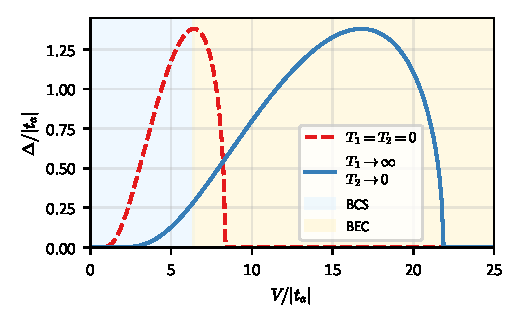
\includegraphics[width=0.5\textwidth]{figures/Gap_V_Tinf_prod_baths.pdf}
    \centering
    \caption{Gap pri $T_1\to \infty$ in $T_2\to 0$.}
\label{pic1}
\end{figure}
\subsection{Fononske sklopitve}
Najprej pogledamo, kako modificiran (Peierls tip) hopping integral in modificiran orbital energy vplivata na sklopitev. Model spremenimo: orbitali znotraj o.c. sta na enakem položaju in se deformirata vedno v isto smer, torej $\vec{u}_{a,i}=\vec{u}_{b,i}=\vec{u}_{i}$. Coulombski potencial se zaradi deformacije ne spremeni veliko. Hamiltonka za nedeformiran kristal ostane enaka, višje člene pa obravnavamo perturbativno: 
\begin{align}
  H[\{\mathbf{u}\}] = \underbrace{\sum_{i, \gamma, \gamma'} \varepsilon_{\gamma\gamma',i}[\{\mathbf{u}\}] \, c_{\gamma,i}^\dagger c_{\gamma',i}^{\vphantom\dagger}}_{\text{on-site in CEF}} + \underbrace{\sum_{\langle i,j \rangle, \gamma} t_{\gamma}(|\mathbf{r}_{ij}|) \, c_{\gamma,i}^\dagger c_{\gamma,j}^{\vphantom\dagger}}_{\text{hopping, med oribitalami}} + \underbrace{V \sum_j n_{a,j} n_{b,j}}_{\text{Coulomb}}
\end{align}
Razdalje so: 
\begin{align}
\vec r_{j}=\vec R_j+\vec u_{j}\,,
\end{align}
oziroma razdalje med paroma (sosedi): 
\begin{align}
\vec r_{ij}=\bm \delta +\vec u_{j} -\vec u_{i}\,\to |\vec r_{ij}| \simeq |\bm \delta| + \bm \delta \cdot (\vec u_{j} -\vec u_{i}) + \mathcal{O}(u^2)
\end{align}
Predpostavimo da na hopping vpliva samo sprememba razdalje:
\begin{align}
  t_{\gamma}(|\mathbf{r}_{ij}|) \simeq t_{\gamma}(|\bm \delta|) + \bm \delta \cdot (\vec u_{j} -\vec u_{i}) \dv{t_\gamma(x)}{x}\bigg|_{x=|\bm\delta|=1}
\end{align} 
Deformacija vpliva na vezavno energijo preko CEF, razvijemo preko deformacijskega tenzorja ($\varepsilon_{\mu\nu}=\frac12(\partial_\mu u_\nu+\partial_\nu u_\mu)$ oziroma diskretno: $\varepsilon_{\mu\nu,j} = \frac14(u_{j+\mu}^\nu-u_{j-\mu}^\nu + u_{j+\nu}^\mu-u_{j-\nu}^\mu)$ zgornji indeks je koordinata vektorja). Če je eno elektronska Hamiltonka na mestu $j$ (el. - ion) (po $\mu, \nu$ se sešteva po Einsteinu): 
\begin{align}
h_j=h_0+\delta h_{j}+O(\varepsilon^2), \quad \delta h_j= \pdv{U_{\text{el-ion}}}{\varepsilon_{\mu \nu,j}}\varepsilon_{\mu \nu,j}, \,(\mu, \nu) = (x, y)
\end{align}
in je v nedeformiranem stanju: 
\begin{align}
  \varepsilon_{\gamma}^{(0)} = \langle \phi_\gamma |h_0|\phi_\gamma \rangle
\end{align}
potem so popravki (lahko mešajo orbitali)
\begin{align} \label{deps_gamgam}
  \delta\varepsilon_{\gamma\gamma'} = \left\langle \phi_\gamma \left|\pdv{U_{\text{el-ion}}}{\varepsilon_{\mu \nu,j}} \right|\phi_{\gamma'} \right\rangle \varepsilon_{\mu \nu,j} = D^{\mu \nu}_{\gamma\gamma'}\varepsilon_{\mu \nu,j}
\end{align}
Sklopitvena Hamiltonka v realni bazi je tako ($\sum_{\langle ij\rangle} \to \sum_i\sum_{\delta=\{x, y\}}$)
\begin{tcolorbox}
\begin{align}
  H_{ep}^{(1)}=\sum_{i, \gamma, \gamma'} D^{\mu \nu}_{\gamma\gamma'}\varepsilon_{\mu \nu,i}  c_{\gamma,i}^\dagger c_{\gamma',i}^{\vphantom\dagger} + \sum_{i, \delta, \gamma} t^\prime_{\gamma} \bm \delta \cdot (\vec u_{i + \delta} -\vec u_{i}) \left(c_{\gamma,i}^\dagger c_{\gamma,i + \delta}^{\vphantom\dagger}  +\text{h.c.}\right)
\end{align}
\end{tcolorbox}
(note):
\begin{align}
     \sum_{\bm{\delta}} \bm{\delta} \cdot (\vec{u}_{i+\delta} - \vec{u}_i) = \hat{x} \cdot (\vec{u}_{i+x} - \vec{u}_i) - \hat{x} \cdot (\vec{u}_{i-x} - \vec{u}_i) + \hat{y} \cdot (\vec{u}_{i+y} - \vec{u}_i) - \hat{y} \cdot (\vec{u}_{i-y} - \vec{u}_i) \approx 2 (\varepsilon_{xx} + \varepsilon_{yy})
\end{align}
Zdaj kvantiziramo odmike in prepišemo v k-prostor, specificno za 2D square lattice: 
\begin{equation}
\vec{u}_j = \frac{1}{\sqrt{N}} \sum_{\vec{q}, \lambda} \frac{1}{\sqrt{2M\omega_{\vec{q}\lambda}}} \bm{\epsilon}_{\vec{q}\lambda} e^{i\vec{q}\cdot\vec{R}_j} \left( b^{\vphantom{\dagger}}_{\vec{q}\lambda} + b_{-\vec{q}\lambda}^\dagger \right)
\end{equation}
v prvem členu so sami členi oblike (od defomracijskega tenzorja, diskretna verzija)
\begin{align} 
  u_{j+\delta}^{\mu}-u_{j-\delta}^{\mu} = \frac{2i}{\sqrt N} \sum_{\vec q,\lambda} \frac{\epsilon_{\vec q\lambda}^{\mu}}{\sqrt{2M\omega_{\vec{q}\lambda}}} \sin(q_\delta)\, e^{i\vec q\cdot\vec R_j} \left( b^{\vphantom{\dagger}}_{\vec{q}\lambda} + b_{-\vec{q}\lambda}^\dagger \right).
\end{align}
v drugem pa členi ($\delta = \mu = \{x, y\}$, glej note):
\begin{align}
  &\frac{t_\gamma'}{\sqrt N} \sum_{\vec q,\vec k',\vec k}  \frac{\epsilon_{\vec q\lambda}^{\mu}}{\sqrt{2M\omega_{\vec{q}\lambda}}} \left( b^{\vphantom{\dagger}}_{\vec{q}\lambda} + b_{-\vec{q}\lambda}^\dagger \right) \left(e^{iq_\mu}-1\right) \left(e^{ik_\mu}+e^{-ik_\mu'}\right) c_{\gamma,\vec k'}^\dagger c_{\gamma,\vec k} \sum_j \frac{1}{N} e^{i(\vec q+\vec k-\vec k')\cdot\vec R_j}  = \\
  &= \frac{t_\gamma'}{\sqrt N} \sum_{\vec k,\vec q} \frac{\epsilon_{\vec q\lambda}^{\mu}}{\sqrt{2M\omega_{\vec{q}\lambda}}} \left( b^{\vphantom{\dagger}}_{\vec{q}\lambda} + b_{-\vec{q}\lambda}^\dagger \right) \left(e^{iq_\mu}-1\right) \left(e^{ik_\mu}+e^{-i(k_\mu+q_\mu)}\right) c_{\gamma,\vec k+\vec q}^\dagger c_{\gamma,\vec k} = \\
  &= \frac{2 i t_\gamma'}{\sqrt N} \sum_{\vec k,\vec q} \frac{\epsilon_{\vec q\lambda}^{\mu}}{\sqrt{2M\omega_{\vec{q}\lambda}}}  \left(\sin(k_\mu + q_\mu)  - \sin(k_\mu)\right) c_{\gamma,\vec k+\vec q}^\dagger c_{\gamma,\vec k} \left( b^{\vphantom{\dagger}}_{\vec{q}\lambda} + b_{-\vec{q}\lambda}^\dagger \right)
\end{align}
Hamiltonka je na koncu oblike (intraband = $\gamma = \gamma'$):
\begin{tcolorbox}
\begin{align}
  H_{ep} = \frac1{\sqrt N} \sum_{\vec k,\vec q,\lambda} \psi_{\vec k+\vec q}^{\dagger} \begin{pmatrix} g_{aa}^{\lambda}(\vec k,\vec q) & g_{ab}^{\lambda}(\vec q)\\ g_{ba}^{\lambda}(\vec q) & g_{bb}^{\lambda}(\vec k,\vec q) \end{pmatrix} \psi_{\vec k} \left( b_{\vec q\lambda}+b_{-\vec q\lambda}^{\dagger} \right)
\end{align}
\begin{align}
   g^\lambda(\vec k,\vec q) = \frac{i}{\sqrt{2M\omega_{\vec q\lambda}}} \begin{pmatrix} 2t_a'T^\lambda(\vec k,\vec q) +{F_{aa}^\lambda(\vec q)} & {F_{ab}^\lambda(\vec q)}\\ {F_{ba}^\lambda(\vec q)} & 2t_b'T^\lambda(\vec k,\vec q) +{F_{bb}^\lambda(\vec q)} \end{pmatrix}.
\end{align}

kjer so: 
\begin{align}
  &T^\lambda(\vec k,\vec q) =\sum_{\mu=x,y}\epsilon_{\vec q\lambda}^{\mu} \left[\sin(k_\mu+q_\mu)-\sin(k_\mu)\right] \\
  &F_{\gamma\gamma'}^\lambda(\vec q) = D_{\gamma\gamma'}^{xx}\epsilon_{\vec q\lambda}^{x}\sin(q_x) + D_{\gamma\gamma'}^{yy}\epsilon_{\vec q\lambda}^{y}\sin(q_y) + D_{\gamma\gamma'}^{xy} \left[ \epsilon_{\vec q\lambda}^{y}\sin(q_x) + \epsilon_{\vec q\lambda}^{x}\sin(q_y)
\right].
\end{align}
\end{tcolorbox}
interband členi so neničelni, glede na izbrane orbitale (glej \eqref{deps_gamgam}) in izbran CF potencial, odvisno od simetrije. Ker smo izbrali $\vec u_{a,i} = \vec u_{b,i}$ se ti elementi sklapljajo samo z akustičnimi fononi, ce znotraj o.c. ni prostostnih stopenj(??). 
\subsection{Optični fononi}
Rabimo dodatne ligande / dodatne ione znotraj celice. Še vedno obdržimo $\vec u_{a,j}=\vec u_{b,j}=\vec u_j$, okolica pa se deformira neodvisno. Odmik liganda $\ell$ v celici $j$ razvijemo po normalnih nacinih
\begin{align}
  \vec v_{j,\ell} = \sum_s Q_{s,j}\, \vec e_{s,\ell}, \qquad \sum_\ell \vec e_{s,\ell}\cdot\vec e_{s',\ell} = \delta_{ss'},
\end{align}
kjer je $s$ indeks nacina, $Q_{s,j}$ skalarna amplituda. Razvijemo enoelektronsko hamiltonko
\begin{align}
  h_j=h_0+\sum_s \pdv{U_{\text{el-ion}}}{Q_{s,j}}\bigg|_{Q=0} Q_{s,j}+O(Q^2), \qquad \Lambda^{s}_{\gamma\gamma'} = \left\langle\phi_\gamma\left| \pdv{U_{\text{el-ion}}}{Q_{s,j}} \right|\phi_{\gamma'}\right\rangle_0 .
\end{align}
\begin{align}
  H_{ep}^{\mathrm{opt}} = \sum_{j, s} \sum_{\gamma, \gamma'} \Lambda^{s}_{\gamma\gamma'} Q_{s,j} \, c_{\gamma,j}^\dagger c_{\gamma',j}^{\vphantom\dagger}.
\end{align}
Kvantiziramo koordinate okoliških ionov:
\begin{align}
  Q_{s,j}= \frac1{\sqrt N} \sum_{\vec q} \frac{1}{\sqrt{2M_s\omega_{\vec q s}}} e^{i\vec q\cdot\vec R_j} \left(b^{\vphantom{\dagger}}_{\vec q s}+b_{-\vec q s}^\dagger\right),
\end{align}
od tod
\begin{align}
  H_{ep}^{\mathrm{opt}} = \frac1{\sqrt N}\sum_{\vec k,\vec q, s} \psi_{\vec k+\vec q}^\dagger \, g^{s}(\vec q) \, \psi_{\vec k} \left(b^{\vphantom{\dagger}}_{\vec q s}+b_{-\vec q s}^\dagger\right), \qquad g^{s}(\vec q) = \frac{\Lambda^{s}}{\sqrt{2M_s\omega_{\vec q s}}}.
\end{align}
% Simetrija določa obliko matrik $\Lambda^s$ (za par orbital s $\phi_a\phi_b\sim xy$):
% \begin{align}
%   \Lambda^{A_{1g}} = \begin{pmatrix} \Lambda_a & 0 \\ 0 & \Lambda_b \end{pmatrix}, \qquad \Lambda^{B_{2g}} = \begin{pmatrix} 0 & \Lambda_{ab} \\ \Lambda_{ab} & 0 \end{pmatrix},
% \end{align}
% za ostale načine je $\Lambda^s = 0$.
Kar da končne sklopitve pri $\vec q \to 0$ ($\Omega_s \equiv \omega_{\vec q\to 0, s}$):
\begin{align}
  g^{s}(\vec q\to0) = \frac{\Lambda^{s}}{\sqrt{2M_s\Omega_s}}.
\end{align}

% \subsubsection{Model prostih elektronov in sklopitev s fononi}
% Razvijemo disperziji
% \begin{equation}
% \varepsilon_{\gamma \vec{k}} = \pm \frac{G}{2} \mp 2t (\cos k_x + \cos k_y) \quad \text{za}\quad k_x, k_y \sim 0
% \end{equation}
% od tod
% \begin{equation}
% \varepsilon_{\gamma \vec{k}} \approx \pm \frac{G}{2} \mp 2t \left( 1 - \frac{k_x^2}{2} + 1 - \frac{k_y^2}{2} \right) = \pm \left( \frac{G}{2} - 4t \right) \pm t (k_x^2 + k_y^2) = \pm (\varepsilon^0 + t \vec{k} \cdot \vec{k})
% \end{equation}
% Torej je Hamiltonka
% \begin{equation}
% H_e^{(0)}  = \sum_{\gamma, \vec{k}} \left( \varepsilon_{\gamma}^0+ t_\gamma {k}^2 \right) c_{\gamma,\vec{k}}^\dagger c_{\gamma,\vec{k}}
% \end{equation}
\subsection{Fotonske sklopitve v resonatorju}
Začnemo z minimalnim modelom za elektrone: 
\begin{align}
  H_e = H_e^{(0)} + H_V = \sum_k \varepsilon_{a,k} c_{a,k}^\dagger c_{a,k} + \sum_k \varepsilon_{b,k} c_{b,k}^\dagger c_{b,k} + V \sum_j c_{a,j}^\dagger c_{a,j} c_{b,j}^\dagger c_{b,j}
\end{align}
in privzamemo 2D plast, kjer sta dve orbitali na o.c., ki hibridizirata samo preko Coulombske interakcije. Disperzije za model neinteragirajoč sistem so v tem primeru enake \eqref{free el tb}. Interakcija pa je v prvem redu oblike: 
\begin{equation}
H_{e\gamma}^{(1)} = -\int \dd{\vec{r}} \, \vec{j}_e \cdot \vec{A} = -\int \dd{\vec{r}} \sum_{\vec{q}} {\vec{A}}({\vec{q}}) e^{i\vec{q}\cdot\vec{r}} \vec{j}_e(\vec{r})  = -\sum_{\vec{q}} {\vec{A}}({\vec{q}}) \cdot \vec{j}_e(\vec{-q})\,,
\end{equation}
kjer je 
\begin{align}
  \vec{A}(\vec{q}) = \sum_\lambda \frac{1}{\sqrt{2\mathcal{V}\epsilon_0 \omega_{\vec{q}, \lambda}}} \bm{\epsilon}_{\vec{q}, \lambda} \left(a_{\vec{q}, \lambda}^{\vphantom{\dagger}} + a_{-\vec{q}, \lambda}^\dagger \right) 
\end{align}
V t.b. modelu dobimo tok iz kontinuitetne in Heisenbergove enačbe: 
\begin{align}
  \frac{\partial \rho(\vec{r})}{\partial t} + \vec{\nabla} \cdot \vec{j} = 0 \, \to\,  i\vec{q} \cdot \vec{j}(\vec{q}) = -\frac{\partial \rho(\vec{q})}{\partial t} 
\end{align}
(+ je od IBP) in 
\begin{equation}
\vec{q}\cdot \vec{j}_e(\vec{q}) = i\frac{\partial \rho(\vec{q})}{\partial t} = -[H_e, \rho(\vec{q})]
\end{equation}
Elektronska gostota je
\begin{equation}
\rho(\vec{r}) = -e \cdot \psi^\dagger(\vec{r}) \psi(\vec{r})
\end{equation}
operatorje polja razvijemo po lokaliziranih / Wannierovih orbitalah
\begin{equation}
\psi(\vec{r}) = \sum_{i,\gamma=\{a, b\}} \phi_\gamma(\vec{r} - \vec{R}_i) c_{\gamma i}\,.
\end{equation}
Transformiramo s FT, uvedemo novo spremenljivko $\vec{r} = \vec{R}_i + \vec{x}$ in razvijemo do dipolov $e^{-i\vec{q}\cdot\vec{x}} \simeq 1 -i\vec{q}\cdot\vec{x}$ (delamo se da se orbitale ne prekrivajo izven o.c., torej $\sum_{ij}\to \sum_{i}\delta_{ij}$): 
\begin{equation}
\rho(\vec{q}) = -e \sum_{i,j} \sum_{\gamma, \gamma'} \int \dd{\vec{r}} \, e^{-i\vec{q}\cdot\vec{r}} \phi_\gamma^*(\vec{r} - \vec{R}_i) \phi_{\gamma'}(\vec{r} - \vec{R}_j) c_{\gamma i}^\dagger c_{\gamma' j} = -e \sum_{i,\gamma,\gamma'} e^{-i\vec{q}\cdot\vec{R}_i} \langle \phi_\gamma | e^{-i\vec{q}\cdot\vec{x}} | \phi_{\gamma'} \rangle c_{\gamma i}^\dagger c_{\gamma' i} 
\end{equation}
Zdaj pa recimo da je dipolni moment samo med različnima orbitalama v o.c. in $n_{\gamma i} = \langle\phi_\gamma |\phi_\gamma\rangle c_{\gamma,i}^\dagger c_{\gamma,i}^ {\vphantom{\dagger}}$:
\begin{equation}
\rho(\vec{q}) \simeq -e \sum_i e^{-i\vec{q}\cdot\vec{R}_i} \left( n_{ai} + n_{bi} - i \vec{q} \cdot \vec{d} \left( c_{a,i}^\dagger c_{b,i}^{\vphantom{\dagger}} + c_{b,i}^\dagger c_{a,i}^{\vphantom{\dagger}} \right) \right)
\end{equation}
zdaj uporabimo zvezo
\begin{equation}
\sum_i e^{i\vec{q}\cdot\vec{R}_i} c_{ai}^\dagger c_{bi} = \sum_{\vec{k}} c_{a, \vec{k}+\vec{q}}^\dagger c_{b\vec{k}}
\end{equation}
z negativnim argumentom je potem elektronska gostota do dipolnega člena (upoštevajoč $\vec{d} = \langle \phi_a(\vec{x}) | \vec{x} | \phi_b(\vec{x}) \rangle$):
\begin{equation}
\rho(-\vec{q}) = -e \sum_{\vec{k}} \begin{pmatrix} c_{a, \vec{k}+\vec{q}}^\dagger & c_{b, \vec{k}+\vec{q}}^\dagger \end{pmatrix} \left( \mathds{1} + i\, \vec{q} \cdot \vec{d} \begin{pmatrix} 0 & 1 \\ 1 & 0 \end{pmatrix} \right) \begin{pmatrix} c_{a\vec{k}} \\ c_{b\vec{k}} \end{pmatrix}
\end{equation}
Zdaj poračunamo komutator, da dobimo tok. Delam z vektorji $\psi_k = \begin{pmatrix} c_{a, \vec{k}} & c_{b, \vec{k}}\end{pmatrix}^\mathsf{T}$: 


\begin{equation}
[H_e^{(0)}, \rho(\vec{q})] =  -e \sum_{\vec{k}, \vec{k'}} \left[ \psi_{\vec{k}}^\dagger \begin{pmatrix} \varepsilon_{a,\vec{k}} & 0 \\ 0 & \varepsilon_{b,\vec{k}} \end{pmatrix} \psi_{\vec{k}}, \psi_{\vec{k'} - \vec{q}}^\dagger \begin{pmatrix} 1 & -i\vec{q}\cdot\vec{d} \\ -i\vec{q}\cdot\vec{d} & 1 \end{pmatrix} \psi_{\vec{k'}} \right]
\end{equation}
uporabimo zvezo:
\begin{align}
  \left[ \psi_{\vec{k}}^\dagger A \psi_{\vec{k}}, \psi_{\vec{k}'-\vec{q}}^\dagger B \psi_{\vec{k}'} \right] &= \psi_{\vec{k}'-\vec{q}}^\dagger \Big( A(\vec{k}'-\vec{q}) B(\vec{k}') - B(\vec{k}'-\vec{q}) A(\vec{k}') \Big) \psi_{\vec{k}'} , \delta_{\vec{k},  \vec{k}'-\vec{q}} \\ &= \psi_{\vec{k}}^\dagger \Big( A(\vec{k}) B(\vec{k}+\vec{q}) - B(\vec{k}) A(\vec{k}+\vec{q}) \Big) \psi_{\vec{k}+\vec{q}}
\end{align}
od tod 
\begin{equation}
\vec{q} \cdot \vec{j}_e(\vec{q}) = -[H_e^{(0)}, \rho(\vec{q})] = -e \sum_{\vec{k}} \psi_{\vec{k}}^\dagger  \begin{pmatrix} \varepsilon_{a,\vec{k}+\vec{q}} - \varepsilon_{a,\vec{k}} & i(\vec{q}\cdot\vec{d})\left(\varepsilon_{a,\vec{k}} - \varepsilon_{b,\vec{k}+\vec{q}}\right) \\ i(\vec{q}\cdot\vec{d})\left(\varepsilon_{b,\vec{k}} - \varepsilon_{a,\vec{k}+\vec{q}}\right) & \varepsilon_{b,\vec{k}+\vec{q}} - \varepsilon_{b,\vec{k}} \end{pmatrix}  \psi_{\vec{k}+\vec{q}}
\end{equation}
da izrazimo tok, naredimo približek, da prispevajo le majhni $\vec{q}\to 0$, zato:
\begin{equation}
\varepsilon_{a, \vec{k}+\vec{q}}- \varepsilon_{a,\vec{k}}   \simeq  \vec{q} \cdot \vec{\nabla}_{\vec{k}} \varepsilon_{\vec{k}+\vec{q}/2}\,,
\end{equation}
kar drži točno za proste elektrone in približno za tight binding disperzije. 
In general ce ne expandamo: 
\begin{align}
  \mathbf{j}_e(\mathbf{q}) = -\frac{e\mathbf{q}}{\Vert{}\mathbf{q}\Vert{}^2} \sum_{\mathbf{k}} \psi_\mathbf{k}^\dagger {M}(\mathbf{k}, \mathbf{q}) \psi_{\mathbf{k}+\mathbf{q}} \;+\; \mathbf{q} \times \mathbf{C}(\mathbf{q})
\end{align}
kjer so $\mathbf{C}(\mathbf{q})$ arbitrarna vektorska polja (tokovi brez divergence, magnetizacijski tokovi). Ce pa naredimo ta priblizek pa dobimo za tok v splošnem, indekse zamaknemo za $-\vec{q}$: 
\begin{tcolorbox}
\begin{equation}
\vec{j}_e(\vec{q}) \simeq -e \sum_{\vec{k}} \psi_{\vec{k}-\vec{q}}^\dagger \begin{pmatrix} \vec{\nabla}_{\vec{k}} \varepsilon_{a,\vec{k}-\vec{q}/2} & i\vec{d}(\varepsilon_{a, \vec{k}-\vec{q}} - \epsilon_{b\vec{k}}) \\ i\vec{d}(\varepsilon_{b, \vec{k}-\vec{q}} - \varepsilon_{a\vec{k}}) & \vec{\nabla}_{\vec{k}} \varepsilon_{b,\vec{k}-\vec{q}/2} \end{pmatrix} \psi_{\vec{k}}\,.
\end{equation}
\end{tcolorbox}
Od tod splošna Hamiltonka v prvem redu:
\begin{tcolorbox}
\begin{align}
H_{e\gamma}^{(1)}
&= -\sum_{\vec{q}} \vec{j}_e(\vec{-q}) \cdot \vec{A}(\vec{q}) = \\
&= \sum_{\vec{k},\vec{q},\lambda} \frac{e}{\sqrt{2\mathcal{V}\varepsilon_0\omega_{\vec{q}, \lambda}}}\, \psi_{\vec{k}+\vec{q}}^\dagger \underbrace{ \begin{pmatrix} \bm{\epsilon}_{\vec{q}\lambda}\cdot \vec{v}_a\!\left(\vec{k}+\frac{\vec{q}}{2}\right) & i\bigl(\bm{\epsilon}_{\vec{q}\lambda}\cdot\vec{d}\bigr) \bigl(\varepsilon_{a,\vec{k}+\vec{q}}-\varepsilon_{b,\vec{k}}\bigr) \\ i\bigl(\bm{\epsilon}_{\vec{q}\lambda}\cdot\vec{d}\bigr) \bigl(\varepsilon_{b,\vec{k}+\vec{q}}-\varepsilon_{a,\vec{k}}\bigr) & \bm{\epsilon}_{\vec{q}\lambda}\cdot \vec{v}_b\!\left(\vec{k}+\frac{\vec{q}}{2}\right) \end{pmatrix} }_{\displaystyle M^\lambda(\vec{k},\vec{q})} \psi_{\vec{k}} \left(a_{\vec{q}\lambda}+a_{-\vec{q}\lambda}^\dagger\right).
\end{align}
\end{tcolorbox}

Za setup od Curtisa: material 2D v $xy$ ravnini, stoječe EM valovanje v $z$, vzamemo osnovni mode ($n=1$), ki prispeva največ, v tem primeru sta dve možni polarizaciji:
\begin{equation}
\vec{\bm{\epsilon}}_{\text{TE}}(z) = \left( \hat{\mathbf{z}} \times \hat{\mathbf{q}} \right) \sin\left(\frac{\pi}{L} z\right)
\end{equation}
\begin{equation}
\vec{\bm{\epsilon}}_{\text{TM}}(z) = \frac{\omega_0}{\omega_{\vec{q}}} \hat{\mathbf{q}} \sin\left(\frac{\pi}{L} z\right) + i \frac{c\, q}{\omega_{\vec{q}}} \hat{\mathbf{z}} \cos\left(\frac{\pi}{L} z\right)
\end{equation}
kjer je $\vec{q} = q(\cos\varphi, \sin\varphi)$ valovni vektor v ravnini, $\omega_0 = \pi c / L$ in $\omega_{\vec{q}} = \sqrt{\omega_0^2 + c^2 q^2}$.
Na sredini resonatorja, pri $z = L/2$, je $\sin(\pi z / L) = 1$ in $\cos(\pi z / L) = 0$, zato:
\begin{equation}
\vec{\bm{\epsilon}}_{\text{TE}}\left(\tfrac{L}{2}\right) = \hat{\mathbf{z}} \times \hat{\mathbf{q}} = \begin{pmatrix} -\sin\varphi \\ \cos\varphi \\ 0 \end{pmatrix}
\end{equation}
\begin{equation}
\vec{\bm{\epsilon}}_{\text{TM}}\left(\tfrac{L}{2}\right) = \frac{\omega_0}{\omega_{\vec{q}}} \hat{\mathbf{q}} = \frac{\omega_0}{\omega_{\vec{q}}} \begin{pmatrix} \cos\varphi \\ \sin\varphi \\ 0 \end{pmatrix}
\end{equation}
Iz tega imamo pri $z = L/2$ možne sklopitve glede na model ($\vec{d} = d(\cos\theta, \sin\theta)$ v ravnini oz. $\vec{d} = d\,\hat{\mathbf{z}}$ izven ravnine):

\begin{table}[h!]
\centering
\begin{tabular}{|l|l|l|l|}
  \hline
\textbf{Nacin} & $\vec{\bm{\epsilon}} \cdot \vec{v}_\gamma\left(\vec{k} + \frac{\vec{q}}{2}\right)$ & $\vec{\bm{\epsilon}} \cdot \vec{d}$, $\vec{d}$ in plane & $\vec{\bm{\epsilon}} \cdot \vec{d}$, $\vec{d} \parallel \hat{\mathbf{z}}$ \\
  \hline

\textbf{TE} & $2 t_\gamma \left( -\sin\varphi \sin\left(k_x + \frac{q_x}{2}\right) + \cos\varphi \sin\left(k_y + \frac{q_y}{2}\right) \right)$ & $d \sin(\theta - \varphi)$ & $0$ \\
  \hline

\textbf{TM} & $\frac{\omega_0}{\omega_{\vec{q}}} 2 t_\gamma \left( \cos\varphi \sin\left(k_x + \frac{q_x}{2}\right) + \sin\varphi \sin\left(k_y + \frac{q_y}{2}\right) \right)$ & $\frac{\omega_0}{\omega_{\vec{q}}} d \cos(\theta - \varphi)$ & $i\, d\, \frac{c\, q}{\omega_{\vec{q}}} \cos\left(\frac{\pi}{L} z\right)$ ($= 0$ pri $z = \frac{L}{2}$) \\
  \hline

\end{tabular}
\end{table}
dipolni moment je neničeln za liho-sode kombinacije orbital in plane, tega gledamo samo glede na o.c.:
\begin{equation}
\vec{d} = \langle \phi_a | \vec{x} | \phi_b \rangle = \int \phi_a^*(\vec{x}) \, \vec{x} \, \phi_b(\vec{x}) \, \dd{\vec{x}}
\end{equation}
\subsubsection{Model prostih elektronov in sklopitev s fotoni}

Kaj pa če gledamo namesto tight binding, proste elektrone, torej 
\begin{equation}
\varepsilon_{\gamma \vec{k}} = \pm \frac{G}{2} \mp 2t (\cos k_x + \cos k_y) \quad \text{za}\quad k_x, k_y \sim 0
\end{equation}
od tod
\begin{equation}
\varepsilon_{\gamma \vec{k}} \approx \pm \frac{G}{2} \mp 2t \left( 1 - \frac{k_x^2}{2} + 1 - \frac{k_y^2}{2} \right) = \pm \left( \frac{G}{2} - 4t \right) \pm t (k_x^2 + k_y^2) = \pm (\varepsilon^0 + t \vec{k} \cdot \vec{k})
\end{equation}
Torej je Hamiltonka
\begin{equation}
H_e^{(0)} = \sum_{\gamma, \vec{k}} \left( \varepsilon_{\gamma}^0+ t_\gamma \vec{k}^2 \right) c_{\gamma,\vec{k}}^\dagger c_{\gamma,\vec{k}}
\end{equation}
Na drug način lahko poračunamo tok, ker razvijemo
\begin{equation}
\psi(\vec{r}) = \frac{1}{\sqrt{\mathcal{V}}}\sum_{\vec{k},\gamma=\{a, b\}}  e^{i \vec{k}\cdot \vec{r}} c_{\gamma, \vec{k}}\,.
\end{equation} 
in za tok uporabimo 
\begin{equation}
\vec{j}_e(\vec{r}) = -\frac{e}{2mi} \left( \psi^\dagger(\vec{r}) \vec{\nabla} \psi(\vec{r}) - \vec{\nabla}\psi^\dagger(\vec{r}) \psi(\vec{r}) \right) = -\frac{e}{2mi} \frac{1}{\mathcal{V}} \sum_{\gamma, \vec{k}, \vec{k}'} \left( c_{\gamma \vec{k}'}^\dagger c_{\gamma \vec{k}} e^{-i\vec{k}'\cdot\vec{r}} (i\vec{k}) e^{i\vec{k}\cdot\vec{r}} - c_{\gamma \vec{k}'}^\dagger c_{\gamma \vec{k}} (-i\vec{k}') e^{-i\vec{k}'\cdot\vec{r}} e^{i\vec{k}\cdot\vec{r}} \right)
\end{equation}
s FT dobimo
\begin{equation}
\vec{j}_e(\vec{-q}) = \int \dd{\vec{r}} \, \vec{j}_e(\vec{r}) e^{i\vec{q}\cdot\vec{r}} = -\frac{e}{2m} \sum_{\gamma, \vec{k}} \left( c_{\gamma, \vec{k}+\vec{q}}^\dagger c_{\gamma \vec{k}} \, \vec{k} + (\vec{k}+\vec{q}) c_{\gamma, \vec{k}+\vec{q}}^\dagger c_{\gamma \vec{k}} \right) = -\frac{e}{m} \sum_{\vec{k}} \left( \vec{k} + \frac{\vec{q}}{2} \right) \psi_{\vec{k}+\vec{q}}^\dagger \psi_{\vec{k}}
\end{equation}
kar bi dobili tudi iz bolj splošne relacije. V tem primeru dobimo enako kot Curtis, $m = 1/2t$
\begin{tcolorbox}
\begin{equation}
H_{e\gamma}^{(1)} = \frac{e}{m} \sum_{\vec{k}, \vec{q}, \lambda}  \frac{1}{\sqrt{2\mathcal{V} \epsilon_0 \omega_{\vec{q}, \lambda}}} \left( \vec{k} + \frac{\vec{q}}{2} \right) \cdot \bm{\epsilon}_{\vec{q}\lambda} \, \psi_{\vec{k}+\vec{q}}^\dagger \psi_{\vec{k}} \left( a_{\vec{q}\lambda} + a_{-\vec{q}\lambda}^\dagger \right)
\end{equation}
\end{tcolorbox}
\subsubsection{Drugi red sklopitve za t.b.}
Zacnemo spet:
\begin{align}
  H_e^{(0)} = \sum_{\gamma, j} \varepsilon_\gamma^{(0)} c_{\gamma j}^\dagger c_{\gamma j}^{\vphantom{\dagger}}- \sum_{j, \bm{\delta}, \gamma} t_\gamma \left( c_{\gamma j}^\dagger c_{\gamma j + \bm{\delta}} + \text{h.c.} \right)
\end{align}
v prisotnosti polja dobi prekrivalni integral fazo: 
\begin{align}
  t_\gamma \to t_\gamma e^{i \theta_{j\bm{\delta}}} \quad\quad \theta_{j\bm{\delta}} = e \int_{\vec{R}_j}^{\vec{R}_j + \bm{\delta}} \vec{A}(\vec{r}, t) \cdot d\vec{r}
\end{align}
od tod
\begin{align}
  H_e^{(0)}[\vec{A}] = \sum_{\gamma, j} \varepsilon_\gamma^{(0)} c_{\gamma j}^\dagger c_{\gamma j}^{\vphantom{\dagger}}- \sum_{j, \bm{\delta}, \gamma} t_\gamma \left( e^{i \theta_{j\bm{\delta}}} c_{\gamma j}^\dagger c_{\gamma j + \bm{\delta}} + e^{-i \theta_{j\bm{\delta}}} c_{\gamma j + \bm{\delta}}^\dagger c_{\gamma j}^{\vphantom{\dagger}}\right)
\end{align}
od kjer razvijemo do drugega reda, prvi red bi moral biti isti kot gor (razen dipolov)
\begin{align}
  e^{i \theta} = 1 + \underbrace{i \theta}_{\mathcal{O}(e\vec{A})} \underbrace{-\frac{1}{2}\theta^2}_{\mathcal{O}(e^2 A^2)}
\end{align}
vstavimo 
\begin{align}
  c_{\gamma j}^{\vphantom{\dagger}}= \frac{1}{\sqrt{\mathcal{V}}} \sum_{\vec{k}} e^{i \vec{k} \cdot \vec{R}_j} c_{\gamma \vec{k}}
\end{align}
in približek da se polje ne spremeni velko do najbližjih sosedov
\begin{align}
  \int_{\vec{R}_j}^{\vec{R}_j + \bm{\delta}} \vec{A}(\vec{r}, t) \cdot d\vec{r} \approx \vec{A}\left(\vec{R}_j + \frac{\bm{\delta}}{2}\right) \cdot \bm{\delta} \quad\quad (\vec{A} \text{\,se ne spremeni veliko znotraj celice+midpoint approx.})
\end{align}
računamo 
\begin{align}
  H_{e\gamma}^{(2)} &= -\sum_{j, \bm{\delta}, \gamma} t_\gamma \left( -\frac{\theta_{j\bm{\delta}}^2}{2} \right) \left( c_{\gamma j}^\dagger c_{\gamma j + \bm{\delta}} + c_{\gamma j + \bm{\delta}}^\dagger c_{\gamma j}^{\vphantom{\dagger}}\right) = \\ &= \sum_{j, \bm{\delta}, \gamma} t_\gamma \cdot \frac{e^2}{2} \int_{\vec{R}_j}^{\vec{R}_j + \bm{\delta}} \vec{A}(\vec{r}, t) \cdot d\vec{r} \int_{\vec{R}_j}^{\vec{R}_j + \bm{\delta}} \vec{A}(\vec{r}, t) \cdot d\vec{r} \left( c_{\gamma j}^\dagger c_{\gamma j + \bm{\delta}} + \text{h.c.} \right) = \\ &= \sum_{j, \bm{\delta}, \gamma} t_\gamma \frac{e^2}{2} \left( \sum_{\vec{q}, \lambda} \frac{1}{\sqrt{2\varepsilon_0 \mathcal{V} \omega_{\vec{q}\lambda}}} \left( \bm{\epsilon}_{\vec{q}\lambda} \cdot \bm{\delta} \right) e^{i \vec{q} \cdot \left(\vec{R}_j + \frac{\bm{\delta}}{2}\right)} \left( a_{\vec{q}\lambda} + a_{-\vec{q}\lambda}^\dagger \right) \right) \left( \sum_{\vec{q}', \lambda'} \frac{1}{\sqrt{2\varepsilon_0 \mathcal{V} \omega_{\vec{q}'\lambda'}}} \left( \bm{\epsilon}_{\vec{q}'\lambda'} \cdot \bm{\delta} \right) e^{i \vec{q}' \cdot \left(\vec{R}_j + \frac{\bm{\delta}}{2}\right)} \left( a_{\vec{q}'\lambda'} + a_{-\vec{q}'\lambda'}^\dagger \right) \right) \\ &\quad \cdot \sum_{\vec{k}, \vec{k}'} \frac{1}{\mathcal{V}} c_{\gamma \vec{k}'}^\dagger c_{\gamma \vec{k}} e^{-i(\vec{k}' - \vec{k}) \cdot \vec{R}_j} \left( e^{i \vec{k} \cdot \bm{\delta}} + e^{i \vec{k}' \cdot \bm{\delta}} \right)
\end{align}
ven pade ohranitev momenta za dvofotonske procese
\begin{align}
  \sum_j \frac{1}{\mathcal{V}} e^{i \left( \vec{q} + \vec{q}' - \vec{k}' + \vec{k} \right) \cdot \vec{R}_j} = \delta_{\vec{k}',\, \vec{k} + \vec{q} + \vec{q}'}
\end{align}
kar da na koncu 
\begin{align}
  = \sum_{\substack{\gamma, \vec{k}, \vec{q}, \vec{q}' \\ \lambda, \lambda', \bm{\delta}}} t_\gamma \frac{e^2}{2} \frac{1}{2\varepsilon_0 \mathcal{V} \sqrt{\omega_{\vec{q}\lambda} \omega_{\vec{q}'\lambda'}}} \left( \bm{\epsilon}_{\vec{q}\lambda} \cdot \bm{\delta} \right) \left( \bm{\epsilon}_{\vec{q}'\lambda'} \cdot \bm{\delta} \right) \left( a_{\vec{q}\lambda} + a_{-\vec{q}\lambda}^\dagger \right) \left( a_{\vec{q}'\lambda'} + a_{-\vec{q}'\lambda'}^\dagger \right) c_{\gamma, \vec{k} + \vec{q} + \vec{q}'}^\dagger c_{\gamma \vec{k}} \\ \cdot \left( e^{i \vec{k} \cdot \bm{\delta}} + e^{-i (\vec{k} + \vec{q} + \vec{q}') \cdot \bm{\delta}} \right) \cdot e^{i (\vec{q} + \vec{q}') \cdot \frac{\bm{\delta}}{2}}
\end{align}
Poenostavimo zadnjifaktor v kosinus:
\begin{tcolorbox}
\begin{align}
  H_{e\gamma}^{(2)} &= \sum_{\substack{\mathbf{k}, \mathbf{q}, \mathbf{q}' \\ \lambda, \lambda'}} \psi_{\mathbf{k}+\mathbf{q}+\mathbf{q}'}^\dagger {M^{\lambda \lambda'}(\mathbf{k}, \mathbf{q}, \mathbf{q}')} \psi_{\mathbf{k}} \cdot (a_{\mathbf{q},\lambda} + a_{-\mathbf{q},\lambda}^\dagger)(a_{\mathbf{q}',\lambda'} + a_{-\mathbf{q}',\lambda'}^\dagger) \\[8pt]
  M^{\lambda \lambda'}(\mathbf{k}, \mathbf{q}, \mathbf{q}') &=  \sum_{\boldsymbol{\delta}} \frac{e^2} {2\varepsilon_0\mathcal V \sqrt{\omega_{\mathbf q,\lambda}\omega_{\mathbf q',\lambda'}}} (\boldsymbol{\epsilon}_{\mathbf{q},\lambda} \cdot \boldsymbol{\delta}) (\boldsymbol{\epsilon}_{\mathbf{q}',\lambda'} \cdot \boldsymbol{\delta})\cos\left(\left(\mathbf{k} + \frac{\mathbf{q}+\mathbf{q}'}{2}\right) \cdot \boldsymbol{\delta}\right) \begin{pmatrix} t_a & 0 \\ 0 & t_b \end{pmatrix}
\end{align}
\end{tcolorbox}
Za n.n. v square latticu eksplicitno: 
\begin{align}
  M^{\lambda\lambda'}(\mathbf k,\mathbf q,\mathbf q') = \frac{e^2} {2\varepsilon_0\mathcal V \sqrt{\omega_{\mathbf q,\lambda}\omega_{\mathbf q',\lambda'}}} \left[ \epsilon_{\mathbf q,\lambda}^{x} \epsilon_{\mathbf q',\lambda'}^{x} \cos\!\left(k_x+\frac{q_x+q_x'}2\right) + \epsilon_{\mathbf q,\lambda}^{y} \epsilon_{\mathbf q',\lambda'}^{y} \cos\!\left(k_y+\frac{q_y+q_y'}2\right) \right] \begin{pmatrix}t_a&0\\0&t_b\end{pmatrix}.
\end{align}

\textbf{A je to consistent z $\mathcal{O}(e\vec A)?$ Če ja, kako dobimo dipole notri v te elemente, al se sam ne sklaplajo nikoli?}
\subsection{Populacijska dinamika}
V splošnem sta za obe bozonski sklopitvi Hamiltonjana oblike (v prvem redu): 
\begin{align}
  H &= \sum_{{\mathbf{k}, \mathbf{q}, \lambda}} \psi_{\mathbf{k}+\mathbf{q}}^\dagger {M^{\lambda}(\mathbf{k}, \mathbf{q})} \psi_{\mathbf{k}} \cdot (a_{\mathbf{q},\lambda} + a_{-\mathbf{q},\lambda}^\dagger)
\end{align}
kar prepišemo v diagonalno bazo za EI s transformacijo \eqref{EI_uintana_rotacija}, za lžje račune definiram v diagonalni bazi: 
\begin{align}
  d_{\gamma, \vec k} = \{\alpha_{\vec{k}}; \gamma=\alpha, \beta_{\vec{k}}; \gamma=\beta\}\,.
\end{align} 
Torej je (indeks veje, oziroma polarizacije $\lambda$ in vsoto bom spuščal v večini primerov):
\begin{align}
  H = \sum_{\substack{\mathbf{k}, \mathbf{q}, \lambda \\ \gamma, \gamma'}} &d_{\gamma,\mathbf{k}+\mathbf{q}}^\dagger {\widetilde{M}_{\gamma,\gamma'}(\mathbf{k}, \mathbf{q})} d_{\gamma', \mathbf{k}} \cdot (a_{\mathbf{q},\lambda} + a_{-\mathbf{q},\lambda}^\dagger)  \\[8pt]
  \widetilde{M}(\mathbf{k}, \mathbf{q}) &= U_{\vec k + \vec{q}}^\dagger M(\mathbf{k}, \mathbf{q}) U_{\vec{k}}
\end{align}
Izpeljava je z von Neumann enačbo, da dobimo pravilne razširjene resonance, na koncu lahko primejamo s Fermijevim zlatim pravilom. Najprej prepišemo Hamiltonjan v interakcijsko sliko v diagonalni bazi je razvoj
\begin{align}
  H_I(t) = \sum_{\substack{\mathbf{k}, \mathbf{q}, \lambda \\ \gamma, \gamma'}} &d_{\gamma,\mathbf{k}+\mathbf{q}}^\dagger {\widetilde{M}_{\gamma,\gamma'}(\mathbf{k}, \mathbf{q})} d_{\gamma', \mathbf{k}} \cdot \left(a_{\mathbf{q},\lambda}(t) + a_{-\mathbf{q},\lambda}^\dagger(t)\right) e^{i\Omega t} \\[8pt]
  \Omega &= E_{\gamma, \vec{k} + \vec q} - E_{\gamma', \vec k}
\end{align}
Sledimo enačbi \eqref{VN-integrated}, kjer zamenjamo $t-s=t'$ in vzamemo $\text{Tr}_S(\hat{n}_{\lambda, \vec p} \bullet)$ na obeh straneh in upoštevamo cikličnost sledi:
\begin{align}
  \partial_t n_{\lambda, \vec p} = - \int_0^t \,\dd{t'}\left\langle \left[\left[d_{\lambda,\mathbf{p}}^\dagger d_{\lambda,\mathbf{p}}, H_I(t)\right], H_I(t')\right]\right\rangle
\end{align}
(note, $\langle\bullet\rangle = \langle\bullet\rangle_S \langle\bullet\rangle_B$) za notranji komutator rabimo:
\begin{align}
  [d_A^\dagger d_B, d_C^\dagger d_D] = d_A^\dagger \underbrace{\{d_B, d_C^\dagger\}}_{\delta_{BC}} d_D - d_C^\dagger \underbrace{\{d_A^\dagger, d_D\}}_{\delta_{AD}} d_B - \underbrace{\{d_A^\dagger, d_C^\dagger\}}_{0} d_B d_D + d_C^\dagger d_A^\dagger \underbrace{\{d_B, d_D\}}_{0}= d_A^\dagger d_D \delta_{BC} - d_C^\dagger d_B \delta_{AD}
\end{align}
oziroma: 
\begin{align}
  [d_A^\dagger d_A, d_C^\dagger d_D] = d_C^\dagger d_D (\delta_{AC} -  \delta_{AD})
\end{align}
Prvi komutator je tako: 
\begin{align}
  [n_{\lambda \vec{p}}, H_{I}(t)] = \sum_{\substack{\vec{k}, \vec{q} \\ \gamma, \gamma'}} \widetilde{M}_{\gamma \gamma'}{(\vec{k}, \vec{q})} \overbrace{d_{\gamma \vec{k}+\vec{q}}^\dagger d_{\gamma' \vec{k}}}^{S} e^{i \Omega t} \overbrace{\left(a_{\vec{q} \lambda} + a_{-\vec{q} \lambda}^\dagger\right)}^{B} \left(\delta_{\lambda \gamma} \delta_{\vec{p}, \vec{k}+\vec{q}} - \delta_{\lambda \gamma'} \delta_{\vec{p}, \vec{k}}\right)
\end{align}
za zunanji komutator nas zanimajo samo operatorji: 
\begin{align}
  \left[ \left[ n_{\lambda \vec{p}}, H_I(t) \right], H_I(t') \right] \sim [S B, S' B'] = S B S' B' - S' B' S B = S S' B B' - S' S B' B
\end{align}  
oziroma bolj natančno (vzamemo še sled, ki se faktorizira za sistem in kopel)
\begin{align}
  \sum_{\substack{{\vec{k}, \vec{q}, \vec{k}', \vec{q}'} \\ {\gamma, \gamma', \omega, \omega'}}}  & \widetilde{M}_{\gamma \gamma'}(\vec{k}, \vec{q}) \widetilde{M}_{\omega \omega'}(\vec{k}', \vec{q}') \left( \delta_{\lambda \gamma} \delta_{\vec{p}, \vec{k}+\vec{q}} - \delta_{\lambda \gamma'} \delta_{\vec{p}, \vec{k}} \right) \cdot \nonumber \\
  & \cdot \Bigg[ \left\langle d_{\gamma \vec{k}+\vec{q}}^\dagger d_{\gamma' \vec{k}}  d_{\omega \vec{k}'+\vec{q}'}^\dagger d_{\omega' \vec{k}'} \right\rangle e^{i \Omega t} e^{i \Omega' t'} \left\langle \left(a_{\vec{q} \lambda} + a_{-\vec{q} \lambda}^\dagger\right)(t) \left(a_{\vec{q}' \lambda'} + a_{-\vec{q}' \lambda'}^\dagger\right)(t') \right\rangle - \nonumber \\
  & - \left\langle d_{\omega \vec{k}'+\vec{q}'}^\dagger d_{\omega' \vec{k}'}  d_{\gamma \vec{k}+\vec{q}}^\dagger d_{\gamma' \vec{k}} \right\rangle e^{i \Omega' t'} e^{i \Omega t} \left\langle \left(a_{\vec{q}' \lambda'} + a_{-\vec{q}' \lambda'}^\dagger\right)(t') \left(a_{\vec{q} \lambda} + a_{-\vec{q} \lambda}^\dagger\right)(t) \right\rangle \Bigg]\,,
\end{align}
kjer je $\Omega' = E_{\omega, \vec k' +\vec{q'}} - E_{\omega', \vec k'} $. Najprej bozonski deli, neničelni so samo mešani produkti (privzel sem še $\omega_\vec{q} = \omega_{-\vec{q}}$):
\begin{align}
  \left\langle \left(a_{\vec q, \lambda} + a_{-\vec q, \lambda}^\dagger\right)(t) \left(a_{\vec{q}', \lambda'} + a_{-\vec{q}', \lambda'}^\dagger\right)(t') \right\rangle &= \left\langle a_{\vec q, \lambda}(t) a_{-\vec{q}', \lambda'}^\dagger(t') \right\rangle + \left\langle a_{-\vec q, \lambda}^\dagger(t) a_{\vec{q}', \lambda'}(t') \right\rangle = \nonumber \\
  &= \left\langle a_{\vec q, \lambda}(t) a_{\vec q, \lambda}^\dagger(t') \right\rangle + \left\langle a_{-\vec q, \lambda}^\dagger(t) a_{-\vec q, \lambda}(t') \right\rangle = \nonumber \\
  &=(N(\omega_{\vec q}) + 1) e^{-i \omega_{\vec q} (t - t')} + N(\omega_{\vec q}) e^{i \omega_{\vec q} (t - t')} 
\end{align}
kjer mora veljati $\vec{q}' = -\vec{q}$ in $\lambda=\lambda'$ (note, ta lambda ni isti kot un fermionski lambda, zmanjkuje mi lepih grskih crk za pisat). Podobno je z drugim členom. Uvedemo še $\tau = t-t'$, integral se ne spremeni z uvedbo te spremenljivke. A la Wick naredimo še za fermionske dele (ker so $d$ diagonalni lahko uporabimo Wicka): 
\begin{align}
  \langle d_A^\dagger d_B d_C^\dagger d_D \rangle &= \langle d_A^\dagger d_B \rangle \langle d_C^\dagger d_D \rangle + \langle d_A^\dagger d_D \rangle \langle d_B d_C^\dagger \rangle = \\
  &= {n_A n_C \delta_{AB} \delta_{CD}} + n_A (1 - n_C) \delta_{BC} \delta_{AD} \\
  &\hookrightarrow \delta_{AB} \mapsto \delta_{\gamma \gamma'} \delta_{\vec{k}+\vec{q}, \vec{k}} = 0 \quad \text{odpade zaradi razlike delta funkcij}
\end{align}
oziroma (prvi člen je nič, ker se nič ne zgodi/ ni sipanje/ga ignoriramo, ker smo fiziki), upoštevamo še $\vec{q}' = -\vec{q}$:
\begin{align}
  \left\langle d_{\gamma \vec{k}+\vec{q}}^\dagger d_{\gamma' \vec{k}} d_{\omega \vec{k}'+\vec{q}'}^\dagger d_{\omega' \vec{k}'} \right\rangle &= n_{\gamma, \vec{k}+\vec{q}} \left(1 - n_{\omega, \vec{k}'-\vec{q}}\right) \delta_{\gamma' \omega} \delta_{\vec{k}, \vec{k}'-\vec{q}} \delta_{\gamma \omega'}  \\ \left\langle d_{\omega \vec{k}'+\vec{q}'}^\dagger d_{\omega' \vec{k}'} d_{\gamma \vec{k}+\vec{q}}^\dagger d_{\gamma' \vec{k}} \right\rangle &= n_{\omega, \vec{k}'-\vec{q}} \left(1 - n_{\gamma, \vec{k}+\vec{q}}\right) \delta_{\omega' \gamma} \delta_{\vec{k}', \vec{k}+\vec{q}} \delta_{\omega \gamma'}
\end{align}
iz delt sledi za eksponenta/časovni razvoj v obeh clenih: 
\begin{align}
  \Omega' = E_{\omega, \vec k' +\vec{q'}} - E_{\omega', \vec k'} = E_{\gamma', \vec k} - E_{\gamma, \vec{k} + \vec q} = - \Omega \implies e^{i \Omega' t'} e^{i \Omega t}  = e^{i \Omega \tau}  
\end{align}
Vse skupaj je treba še integrirati, dodamo regulator, da pole izmaknemo iz osi: 
\begin{align}
  \int_{0}^{\infty} e^{i \tau (\Omega \pm \omega_{\vec q} + i\gamma)} \, d\tau = -\frac{i e^{i(\Omega \pm \omega_{\vec q})\tau} e^{-\gamma \tau}}{\Omega \pm \omega_{\vec q} + i\gamma} \bigg\vert_{0}^{\infty} = \frac{i}{\Omega \pm \omega_{\vec q} + i\gamma} = D_{\pm}(\Omega)
\end{align}
oziroma skupaj: 
\begin{align}
  \partial_t n_{\lambda, \vec p} &= -\int_{0}^{t\to \infty} \sum_{\substack{\vec{k}, \vec{q} \\ \gamma, \gamma'}} \left(\delta_{\lambda \gamma} \delta_{\vec{p}, \vec{k}+\vec{q}} - \delta_{\lambda \gamma'} \delta_{\vec{p}, \vec{k}}\right) \cdot \\ 
  \cdot &\left( n_{\gamma, \vec{k}+\vec{q}} (1 - n_{\gamma', \vec{k}}) \widetilde{M}_{\gamma \gamma'}{(\vec{k}, \vec{q})} \widetilde{M}_{\gamma' \gamma}(\vec{k}+\vec{q}, -\vec{q}) e^{i \Omega \tau} \left( (N(\omega_{\vec q}) + 1) e^{-i \omega_{\vec q} \tau} + N(\omega_{\vec q}) e^{i \omega_{\vec q} \tau} \right) \right. \\ &\left. - \; n_{\gamma', \vec{k}} (1 - n_{\gamma, \vec{k}+\vec{q}}) \widetilde{M}_{\gamma \gamma'}{(\vec{k}, \vec{q})} \widetilde{M}_{\gamma' \gamma}{(\vec{k}+\vec{q}, -\vec{q})} e^{i \Omega \tau} \left( (N(\omega_{\vec q}) + 1) e^{i \omega_{\vec q} \tau} + N(\omega_{\vec q}) e^{-i \omega_{\vec q} \tau} \right) \right) \, \dd{\tau}
\end{align}
Iz hermitskosti sledi: 
\begin{align}
    \widetilde{M}_{\gamma' \gamma}(\vec{k}+\vec{q}, -\vec{q}) = \widetilde{M}_{\gamma' \gamma}{(\vec{k}, \vec{q})}^*
\end{align}
ko razpišemo vseh 8 členov z deltami in preimenujemo indekse ostane ($\Omega =  E_{\lambda, \vec p} - E_{\gamma, \vec k}$)
\begin{align}
   \partial_t n_{\lambda, \vec p} = -\sum_{\vec{k}, \gamma} \left\vert{} \widetilde{M}_{\gamma \lambda} \right\vert{}^2 n_{\lambda \vec{p}} (1 - n_{\gamma \vec{k}}) \left\{ (N_{\vec{p}-\vec{k}} + 1) \left[ D_-(\Omega) + D_+(-\Omega) \right] + N_{\vec{p}-\vec{k}} \left[ D_+(\Omega) + D_-(-\Omega) \right] \right\} + \\ + \sum_{\vec{k}, \gamma} \left\vert{} \widetilde{M}_{\lambda \gamma} \right\vert{}^2 (1 - n_{\lambda \vec{p}}) n_{\gamma \vec{k}} \left\{ (N_{\vec{p}-\vec{k}} + 1) \left[ D_+(\Omega) + D_-(-\Omega) \right] + N_{\vec{p}-\vec{k}} \left[ D_-(\Omega) + D_+(-\Omega) \right] \right\} 
\end{align}
od kjer lahko poenostavimo: 
\begin{align}
  D_-(\Omega) + D_+(-\Omega) = \frac{2\gamma}{(\Omega - \omega_{\vec{q}})^2 + \gamma^2} \equiv \mathcal{A}_{\vec q}(\Omega) \\
  D_+(\Omega) + D_-(-\Omega) = \frac{2\gamma}{(\Omega + \omega_{\vec{q}})^2 + \gamma^2} = \mathcal{A}_{\vec q}(-\Omega) 
\end{align}
oziroma končno:; 
\begin{tcolorbox}
\begin{align}
\partial_t {n}_{\gamma \vec{k}} &= \sum_{\vec{k}', \gamma'} \Gamma_{\gamma' \vec{k}' \to \gamma \vec{k}} n_{\gamma' \vec{k}'} (1 - n_{\gamma \vec{k}}) - \Gamma_{\gamma \vec{k} \to \gamma' \vec{k}'} n_{\gamma \vec{k}} (1 - n_{\gamma' \vec{k}'}) \\ \Gamma_{\gamma' \vec{k}' \to \gamma \vec{k}} &= \sum_{\lambda} \left\vert{} \tilde{M}^{\lambda}_{\gamma \gamma'}(\vec{k}', \vec{k} -\vec{k}') \right\vert{}^2 \cdot \Big\{ (N_\lambda(-\Omega) + 1) \mathcal{A}_{\vec{k}-\vec{k}', \lambda}(-\Omega) + N_\lambda(\Omega) \mathcal{A}_{\vec{k}-\vec{k}', \lambda}(\Omega) \Big\} \\ \Gamma_{\gamma \vec{k} \to \gamma' \vec{k}'} &= \sum_{\lambda} \left\vert{} \tilde{M}^{\lambda}_{\gamma \gamma'}(\vec{k}', \vec{k} - \vec{k}') \right\vert{}^2 \cdot \Big\{ (N_\lambda(\Omega) + 1) \mathcal{A}_{\vec{k}'-\vec{k}, \lambda}(\Omega) + N_\lambda(-\Omega) \mathcal{A}_{\vec{k}'-\vec{k}, \lambda}(-\Omega) \Big\} \\ \Omega &= E_{\gamma \vec{k}} - E_{\gamma' \vec{k}'}, \qquad N(-\Omega) = -1 - N(\Omega)
\end{align}
\end{tcolorbox} \noindent
preverimo predznake v tabeli \ref{tabela_feynman}.

\begin{table}[ht] 
  \centering  
  \setlength{\tabcolsep}{8pt}
  \begin{tabular}{|c|c|}
    \hline
    \begin{minipage}[t]{0.45\textwidth}
      \centering
      \vspace{8pt}
      \(\mathrm{A}1\)\par\medskip
      \dg{(v) -- [charged boson] (q)}
         {\vec q=\vec k-\vec k'}
         {\vec k,\gamma}{\vec k',\gamma'}{}
      \[
        \begin{aligned}
          \Omega+\omega_{\vec q}&\simeq0\\
          &=E_{\gamma\vec k}-E_{\gamma'\vec k'}+\omega_{\vec q}\\
          &=\underbrace{(E_{\gamma\vec k}+\omega_{\vec q})}_{E_f}
            -\underbrace{E_{\gamma'\vec k'}}_{E_i}.
        \end{aligned}
      \]
      \vspace{4pt}
    \end{minipage}
    &
    \begin{minipage}[t]{0.45\textwidth}
      \centering
      \vspace{8pt}
      \(\mathrm{A}2\)\par\medskip
      \dg{(q) -- [charged boson] (v)}
         {\vec q=\vec k-\vec k'}
         {\vec k,\gamma}{\vec k',\gamma'}{}
      \[
        \begin{aligned}
          \Omega-\omega_{\vec q}&\simeq0\\
          &=E_{\gamma\vec k}-E_{\gamma'\vec k'}-\omega_{\vec q}\\
          &=\underbrace{E_{\gamma\vec k}}_{E_f}
            -\underbrace{(E_{\gamma'\vec k'}+\omega_{\vec q})}_{E_i}.
        \end{aligned}
      \]
      \vspace{4pt}
    \end{minipage}
    \\
    \hline
    \begin{minipage}[t]{0.45\textwidth}
      \centering
      \vspace{8pt}
      \(\mathrm{B}1\)\par\medskip
      \dg{(v) -- [charged boson] (q)}
         {\vec q=\vec k'-\vec k}
         {\vec k',\gamma'}{\vec k,\gamma}{\,|M|^2}
      \[
        \begin{aligned}
          \Omega-\omega_{\vec q}&\simeq0\\
          &=E_{\gamma\vec k}-E_{\gamma'\vec k'}-\omega_{\vec q}\\
          &=-\bigl[(E_{\gamma'\vec k'}+\omega_{\vec q})
                    -E_{\gamma\vec k}\bigr].
        \end{aligned}
      \]
      \vspace{4pt}
    \end{minipage}
    &
    \begin{minipage}[t]{0.45\textwidth}
      \centering
      \vspace{8pt}
      \(\mathrm{B}2\)\par\medskip
      \dg{(q) -- [charged boson] (v)}
         {\vec q=\vec k'-\vec k}
         {\vec k',\gamma'}{\vec k,\gamma}{}
      \[
        \begin{aligned}
          \Omega+\omega_{\vec q}&\simeq0\\
          &=E_{\gamma\vec k}-E_{\gamma'\vec k'}+\omega_{\vec q}\\
          &=-\bigl[E_{\gamma'\vec k'}
                    -(E_{\gamma\vec k}+\omega_{\vec q})\bigr].
        \end{aligned}
      \]
      \vspace{4pt}
    \end{minipage}
    \\
    \hline
  \end{tabular}
  \caption{Feynman diagrami za vse štiri procese (iz in v fiskno stanje $\gamma, \vec k$).}
  \label{tabela_feynman}
\end{table}

Dobimo enako kot Curtis, čeprav smo fotone obravnavali v približku: za korelatorje oziroma produkte bozonov smo privzeli da imajo točno definirane resonance in dodali regulator na roke. V resnici so fotoni sklopljeni z okolico, kar jim da končno širino v disperziji. Rate matrike lahko še porenostavimo na razlike Lotentzovih vrhov: 
\begin{align}
  \Gamma_{\gamma' \vec{k}' \to \gamma \vec{k}} &= | \widetilde{M}_{\gamma \gamma'}(\vec{k}', \vec{k} -\vec{k}') |^2 N(\Omega) \cdot \Big\{\mathcal{A}_{\vec{k}-\vec{k}'}(\Omega) - \mathcal{A}_{\vec{k}-\vec{k}'}(-\Omega) \Big\} \\ \Gamma_{\gamma \vec{k} \to \gamma' \vec{k}'} &= | \widetilde{M}_{\gamma \gamma'}(\vec{k}', \vec{k} - \vec{k}') |^2 (N(\Omega) + 1) \cdot \Big\{ \mathcal{A}_{\vec{k}'-\vec{k}}(\Omega) - \mathcal{A}_{\vec{k}'-\vec{k}}(-\Omega) \Big\} 
\end{align} 
od kjer vidimo, da s tem točno zadostimo detaljnemu ravnovesju(?nevem kaj je prevod): 
\begin{align}
  \frac{\Gamma_{\gamma' \vec{k}' \to \gamma \vec{k}}}{\Gamma_{\gamma \vec{k} \to \gamma' \vec{k}'}} = \frac{N(\Omega) }{N(\Omega)  +1} = e^{-\Omega /  T}\,.
\end{align}
Če vzamemo GGE obliko, za boljšo stabilnost: $n_{\gamma \vec{k}} = 1/(1+\exp(\mu_{\gamma \vec k}))$, potem je 
\begin{align}
  \partial_t n_{\gamma \vec{k}} = -n_{\gamma \vec{k}} (1 - n_{\gamma \vec{k}}) \partial_t \mu_{\gamma \vec{k}} = \mathcal{I}_{\gamma \vec{k}}
\end{align}
\begin{align}
  \mathcal{I}_{\gamma \vec{k}} = \sum_{\gamma', \vec{k}'} \left[ \Gamma_{\gamma' \vec{k}' \to \gamma \vec{k}} (1 - n_{\gamma \vec{k}}) n_{\gamma' \vec{k}'} -  \Gamma_{\gamma \vec{k} \to \gamma' \vec{k}'} (1 - n_{\gamma' \vec{k}'}) n_{\gamma \vec{k}} \right]
\end{align}
\begin{align}
  \partial_t \mu_{\gamma \vec{k}} = -\frac{\mathcal{I}_{\gamma \vec{k}}}{n_{\gamma \vec{k}} (1 - n_{\gamma \vec{k}})}
\end{align}
oziroma: 
\begin{align}
  \partial_t \mu_{\gamma \vec{k}} = -\sum_{\gamma', \vec{k}', b} \Gamma_{\gamma' \vec{k}' \to \gamma \vec{k}}^{b} \frac{1 + e^{\mu_{\gamma \vec{k}}}}{1 + e^{\mu_{\gamma' \vec{k}'}}} - \Gamma_{\gamma \vec{k} \to \gamma' \vec{k}'}^{b} \frac{1 + e^{-\mu_{\gamma \vec{k}}}}{1 + e^{-\mu_{\gamma' \vec{k}'}}}\,,
\end{align}
kjer je $\Gamma^{b}=\Gamma(T_b)$. Izraz se poenostavi če upoštevamo še zahtevo po d.b.: 
\begin{tcolorbox}
  \begin{align}
    \partial_t \mu_{\gamma \vec{k}} = \sum_{\gamma' \vec{k}', b} \Gamma_{\gamma' \vec{k}' \to \gamma \vec{k}}^b \frac{1 + e^{\mu_{\gamma \vec{k}}}}{1 + e^{\mu_{\gamma' \vec{k}'}}} \left(e^{\Omega / T_b + \mu_{\gamma' \vec{k}'} - \mu_{\gamma \vec{k}}} - 1\right)
  \end{align}
\end{tcolorbox}
\subsection{Sprememba koordinat} 
Za 2D square lattice mrežo uvedemo: 
\begin{align}
s=\cos k_x+\cos k_y,\qquad
u=\cos k_x-\cos k_y.
\end{align}
Obratna transformacija je bijektivna na irreducible trikotniku ($\Gamma -X-M$, oziroma: $\{(k_x,k_y):0\leq k_y\leq k_x\leq\pi\}$):
\begin{align}
  \vec{k}(s,u) = \left(\arccos\!\left(\frac{s+u}{2}\right), \arccos\!\left(\frac{s-u}{2}\right)\right)^\mathsf{T}
\end{align}
Z nekaj obračanja dobimo območje kjer sta definirani novi spremenljivki: 
\begin{align}
-2\leq s\leq2,\qquad |s|-2\leq u\leq0
\end{align}
\begin{align}
\varepsilon_a(s)=\frac G2-2t_a s,\qquad
\varepsilon_b(s)=-\frac G2-2t_b s.
\end{align}
\begin{align}
\varepsilon_a^H(s)
&=\frac G2-2t_a s+\frac V2(n-m),\\
\varepsilon_b^H(s)
&=-\frac G2-2t_b s+\frac V2(n+m).
\end{align}
\begin{align}
\eta(s)
&=\frac{\varepsilon_a^H(s)+\varepsilon_b^H(s)}2
=\frac{Vn}{2}-(t_a+t_b)s,\\
\xi(s)
&=\frac{\varepsilon_a^H(s)-\varepsilon_b^H(s)}2
=\frac{G-Vm}{2}-(t_a-t_b)s.
\end{align}

\begin{align}
E_{\alpha,\beta}(s,u)=
\frac{Vn}{2}-(t_a+t_b)s
\ \pm\
\sqrt{
\left[\frac{G-Vm}{2}-(t_a-t_b)s\right]^2+|\Delta|^2
}.
\end{align}
\begin{align}
u_{\vec k} \to u^2(s)
&={\frac12\left(1+\frac{\xi(s)}{\sqrt{\xi^2(s)+\Delta^2}}\right)},\\
v_{\vec k} \to v^2(s)
&={\frac12\left(1-\frac{\xi(s)}{\sqrt{\xi^2(s)+\Delta^2}}\right)},\\
u_{\vec k}v_{\vec k} \to u(s)v(s)
&=-\frac{\Delta}{2\sqrt{\xi^2(s)+\Delta^2}}.
\end{align}
Za integrale/fazne vsote po 1. B.C. je Jakobijan
\begin{align}
\left|\frac{\partial(s,u)}{\partial(k_x,k_y)}\right|
=2\sin k_x\sin k_y.
\end{align}
Za intergal po 1. B.C. lahko v najbolj simetričnem primeru (za funckijo $F(g\vec{k}) = F(\vec{k})\,,\forall g\in C_{4v}$) pišemo (upoštevamo integral po trikotniku $\cdot 8$)
\begin{align}
\langle F\rangle_{\mathrm{B.C.}}
=\frac{1}{(2\pi)^2}\int_{\mathrm{B.C.}}d^2k\,F(\vec k) =\frac1{\pi^2}
\int_{-2}^{2}ds\int_{|s|-2}^{0}du\,
\frac{F(s,u)}
{\sqrt{1-\frac{(s+u)^2}{4}}\,
 \sqrt{1-\frac{(s-u)^2}{4}}}.
\end{align}
Velikokrat je $F(s, u) = F(s)$, takrat velja: 
\begin{align}
  \pi^2  g(s)= \int_{\vert{}s\vert{}-2}^{0} du \frac{1}{\sqrt{1 - \frac{(s+u)^2}{4}} \sqrt{1 - \frac{(s-u)^2}{4}}} = \frac{4}{2+\vert{}s\vert{}} K\left( \frac{2-\vert{}s\vert{}}{2+\vert{}s\vert{}} \right) 
\end{align}
\begin{align}
  K(k) = \int_{0}^{\pi/2} \frac{d\theta}{\sqrt{1 - k^2 \sin^2\theta}}
\end{align}
okoli $s \approx 0:$
\begin{align}
  \pi^2 g(s) \approx (2-\vert{}s\vert{}) \cdot \frac{1}{2} \ln\left(\frac{8}{\vert{}s\vert{}}\right) \approx \ln\left(\frac{8}{\vert{}s\vert{}}\right)
\end{align}
\begin{align}
  \langle F \rangle_{\text{B.C.}} = \int_{-2}^{2} g(s) \cdot F(s) \, ds \quad ; \quad g(s) = \frac{1}{\pi^2} \frac{4}{2+\vert{}s\vert{}} K\left( \frac{2-\vert{}s\vert{}}{2+\vert{}s\vert{}} \right)
\end{align}
V termičnem primeru velja: 
\begin{align}
\Delta
&=V\left\langle
\frac{\Delta}{2\sqrt{\xi^2(s)+\Delta^2}}[f_\beta(s)-f_\alpha(s)]
\right\rangle_{\mathrm{B.C.}},\\
m
&=\left\langle
\frac{\xi(s)}{\sqrt{\xi^2(s)+\Delta^2}}[f_\alpha(s)-f_\beta(s)]
\right\rangle_{\mathrm{B.C.}},\\
n
&=\left\langle f_\alpha(s)+f_\beta(s)\right\rangle_{\mathrm{B.C.}}.
\end{align}
Za najbolj splošen primer je integral enak:
\begin{align}
\langle F(\vec{k})\rangle_{\mathrm{B.C.}} =
&=\frac1{8\pi^2} \sum_{g\in C_{4v}}
\int_{-2}^{2}ds\int_{|s|-2}^{0}du\,
\frac{F(g\vec{k}(s, u))}
{\sqrt{1-\frac{(s+u)^2}{4}}\,
 \sqrt{1-\frac{(s-u)^2}{4}}}\,.
\end{align}
Najprej opazimo da je za $g \in C_{4v}$ spremeljivka $s$ in vse količine, ki so samo funkcije $s$ invariantna, spremeljivka $u$ pa se transfromira kot $u \to u\,, g=\{E, C_2, \sigma_v, \sigma_{v'}\}$ in $u \to -u$ za ostale 4 elemente. Torej, če je $F(s, u)$ soda v $u$ je invariantna, v splošnem pa je:
\begin{align}
  \sum_{g\in C_{4v}} F(g\vec{k}) = 4 F(s, u) + 4F(s, -u)\,.
\end{align}
zato je v splošnem: 
\begin{tcolorbox}
  \begin{align}
    \langle F(\vec{k})\rangle_{\mathrm{B.C.}} =\frac1{2\pi^2} \int_{-2}^{2}ds\int_{|s|-2}^{0}du\, \frac{F(s, u) + F(s, -u)} {\sqrt{1-\frac{(s+u)^2}{4}}\,  \sqrt{1-\frac{(s-u)^2}{4}}}\,.
  \end{align}
\end{tcolorbox}
Za netermični primer je rahla komplikacija z $f_\gamma(s)\mapsto n_\gamma(s, u)$. Prepisati moramo sipalni integral  $\mathcal{I}_{\gamma \vec{k}}$ na nove spremenljivke. 
\begin{align}
\partial_t \mu_{\gamma \vec{k}} &= \sum_{\gamma', b} \frac{1}{2\pi^2} \int_{-2}^{2}ds'\int_{|s|-2}^{0}du' \, J(s', u') \sum_{i=1}^{2} \left[ {\Gamma}_{\gamma' \vec{k}'_i \to \gamma \vec{k}}^b \frac{1 + e^{\mu_{\gamma \vec{k}}}}{1 + e^{\mu_{\gamma' \vec{k}'_i}}} \left(e^{\Omega / T_b + \mu_{\gamma' \vec{k}'_i} - \mu_{\gamma \vec{k}}} - 1\right) \right] \\
{\Gamma}_{\gamma' \vec{k}'_i \to \gamma \vec{k}}^b &= \vert{}\widetilde{M}_{\gamma \gamma'}(\vec{k}'_i, \vec{k} - \vec{k}'_i)\vert{}^2 N(\Omega) \cdot \Big\{\mathcal{A}_{\vec{k} - \vec{k}'_i}(\Omega) - \mathcal{A}_{\vec{k} - \vec{k}'_i}(-\Omega)\Big\} \\
\vec{k}'_1 &= \vec{k}'(s', u')\,,\quad \vec{k}'_2 = \vec{k}'(s', -u')
\end{align}
kjer 
\begin{align}
  \vec{k}'_1 &= \left( k_{x1}', \, k_{y1}' \right) = \left( \arccos\left(\frac{s' + u'}{2}\right), \, \arccos\left(\frac{s' - u'}{2}\right) \right) \\
  \vec{k}'_2 &= \left( k_{x2}', \, k_{y2}' \right) = \left( \arccos\left(\frac{s' - u'}{2}\right), \, \arccos\left(\frac{s' + u'}{2}\right) \right)
\end{align}
če je $\Gamma$ popolnoma simetrična na vse operacije vsaj vemo, da je $\mu_\gamma(s, u) = \mu_\gamma(s, -u)$, ne določa pa to odvisnosti od $u$. Recimo, da fiksiramo $\omega_\vec{q} = \sqrt{\omega_0^2+c^2q^2}$. Ta je invariantna na $C_{4v}$,  tudi $\Omega= \Omega(s)$ je, zato je $\mathcal{A}_\vec{q}(\Omega)$ invariantna. Enako velja za Bose faktorje. 

\section{Konkretna implementacija za sklopitev s fotoni}
konkretna implementacija/racun za verteks za fotone: 
% k: final momentum, k': initial momentum, q = k - k' wrapped to the first BZ, a_0 = 1
\begin{align}
\mathbf{q} &= q(\cos\varphi,\sin\varphi), \qquad
\varphi = \operatorname{atan2}(q_y,q_x)\ (\varphi=0\,\, \text{pri}\,\, \mathbf{q}=0), \qquad
\omega_{\mathbf{q}} = \sqrt{\omega_0^2 + c^2 q^2},\\
s_{\mathbf{k}} &= \cos k_x + \cos k_y, \qquad
\varepsilon_{a,\mathbf{k}} = \tfrac{G}{2} - 2t_a s_{\mathbf{k}}, \qquad
\varepsilon_{b,\mathbf{k}} = -\tfrac{G}{2} - 2t_b s_{\mathbf{k}} .
\end{align}
% velocity of band gamma = a, b from eq. 21, a_0 = 1
\begin{equation}
\mathbf{v}_{\gamma}(\mathbf{p}) = \nabla_{\mathbf{p}}\,\varepsilon_{\gamma,\mathbf{p}}
= \nabla_{\mathbf{p}}\left[\pm\tfrac{G}{2} - 2t_\gamma(\cos p_x + \cos p_y)\right]
= 2t_\gamma\,(\sin p_x,\ \sin p_y) .
\end{equation}

% evaluated at the midpoint p = k' + q/2 (eq. 125)
\begin{equation}
\mathbf{v}_{\gamma}\!\left(\mathbf{k}'+\tfrac{\mathbf{q}}{2}\right) = 2t_\gamma\,(\sin\!\left(k'_x + \tfrac{q_x}{2}\right),\ \sin\!\left(k'_y + \tfrac{q_y}{2}\right)),
\end{equation}

% so the diagonal elements of eq. 125 are
\begin{equation}
\boldsymbol{\epsilon}_{\lambda}\cdot\mathbf{v}_{\gamma}\!\left(\mathbf{k}'+\tfrac{\mathbf{q}}{2}\right)
= 2t_\gamma\,X_\lambda, \qquad
X_\lambda = \boldsymbol{\epsilon}_{\lambda}\cdot(\sin\!\left(k'_x + \tfrac{q_x}{2}\right),\ \sin\!\left(k'_y + \tfrac{q_y}{2}\right)) .
\end{equation}
% polarizations at z = L/2 and dipole along x
\begin{align}
\boldsymbol{\epsilon}_{\mathrm{TE}} &= (-\sin\varphi,\ \cos\varphi), &
\boldsymbol{\epsilon}_{\mathrm{TM}} &= \frac{\omega_0}{\omega_{\mathbf{q}}}(\cos\varphi,\ \sin\varphi), &
\mathbf{d} &= d\,(1,0).
\end{align}

% scalar projections, with h_x = sin(k'_x + q_x/2), h_y = sin(k'_y + q_y/2)
\begin{align}
X_{\mathrm{TE}} &= -\sin\varphi\, h_x + \cos\varphi\, h_y, &
X_{\mathrm{TM}} &= \frac{\omega_0}{\omega_{\mathbf{q}}}\left(\cos\varphi\, h_x + \sin\varphi\, h_y\right),\\
P_{\mathrm{TE}} &= -d\sin\varphi, &
P_{\mathrm{TM}} &= \frac{\omega_0}{\omega_{\mathbf{q}}}\, d\cos\varphi,
\end{align}
\begin{align}
\Delta_{ab} &= \varepsilon_{a,\mathbf{k}} - \varepsilon_{b,\mathbf{k}'} = G - 2t_a s_{\mathbf{k}} + 2t_b s_{\mathbf{k}'}, &
\Delta_{ba} &= \varepsilon_{b,\mathbf{k}} - \varepsilon_{a,\mathbf{k}'} = -G - 2t_b s_{\mathbf{k}} + 2t_a s_{\mathbf{k}'} .
\end{align}

% orbital vertex (eq. 125), g_q^2 = A / omega_q with A = amp
\begin{equation}
M^{\lambda}(\mathbf{k}',\mathbf{q}) = \sqrt{\frac{A}{\omega_{\mathbf{q}}}}
\begin{pmatrix}
2t_a X_\lambda & i P_\lambda \Delta_{ab}\\
i P_\lambda \Delta_{ba} & 2t_b X_\lambda
\end{pmatrix}
\end{equation}

% rotation (eq. 32, 157); u, v at k and u', v' at k'
\begin{equation}
\widetilde{M}^{\lambda} = U_{\mathbf{k}}^{T} M^{\lambda} U_{\mathbf{k}'}, \qquad
U_{\mathbf{k}} = \begin{pmatrix} u & v\\ -v & u \end{pmatrix}, \qquad
u = \sqrt{\tfrac12\left(1+\tfrac{\xi_{\mathbf{k}}}{E_{\mathbf{k}}}\right)}, \quad
v = \operatorname{sgn}(\Delta)\sqrt{\tfrac12\left(1-\tfrac{\xi_{\mathbf{k}}}{E_{\mathbf{k}}}\right)} .
\end{equation}

\begin{align}
\widetilde{M}^{\lambda}_{\alpha\alpha} &= \sqrt{\frac{A}{\omega_{\mathbf{q}}}} \left[ X_\lambda\,(2t_a uu' + 2t_b vv') - i P_\lambda\,(uv'\Delta_{ab} + vu'\Delta_{ba}) \right],\\
\widetilde{M}^{\lambda}_{\alpha\beta} &= \sqrt{\frac{A}{\omega_{\mathbf{q}}}} \left[ X_\lambda\,(2t_a uv' - 2t_b vu') + i P_\lambda\,(uu'\Delta_{ab} - vv'\Delta_{ba}) \right],\\
\widetilde{M}^{\lambda}_{\beta\alpha} &= \sqrt{\frac{A}{\omega_{\mathbf{q}}}} \left[ X_\lambda\,(2t_a vu' - 2t_b uv') + i P_\lambda\,(uu'\Delta_{ba} - vv'\Delta_{ab}) \right],\\
\widetilde{M}^{\lambda}_{\beta\beta} &= \sqrt{\frac{A}{\omega_{\mathbf{q}}}} \left[ X_\lambda\,(2t_a vv' + 2t_b uu') + i P_\lambda\,(vu'\Delta_{ab} + uv'\Delta_{ba}) \right].
\end{align}

% the velocity part is real and the dipole part imaginary, so there is no cross term
\begin{align}
\sum_{\lambda}\left|\widetilde{M}^{\lambda}_{\gamma\gamma'}\right|^2
&= \frac{A}{\omega_{\mathbf{q}}}\left[
\left(X_{\mathrm{TE}}^2 + X_{\mathrm{TM}}^2\right) C_{\gamma\gamma'}^2
+ \left(\sin^2\varphi + \frac{\omega_0^2}{\omega_{\mathbf{q}}^2}\cos^2\varphi\right) D_{\gamma\gamma'}^2 \right]\,,\\
C_{\alpha\alpha} &= 2t_a uu' + 2t_b vv', & D_{\alpha\alpha} &= d\,(uv'\Delta_{ab} + vu'\Delta_{ba}),\\
C_{\alpha\beta} &= 2t_a uv' - 2t_b vu', & D_{\alpha\beta} &= d\,(uu'\Delta_{ab} - vv'\Delta_{ba}),\\
C_{\beta\alpha} &= 2t_a vu' - 2t_b uv', & D_{\beta\alpha} &= d\,(uu'\Delta_{ba} - vv'\Delta_{ab}),\\
C_{\beta\beta} &= 2t_a vv' + 2t_b uu', & D_{\beta\beta} &= d\,(vu'\Delta_{ab} + uv'\Delta_{ba}).
\end{align}

% rate (eq. 186), Omega = E_{gamma k} - E_{gamma' k'}
\begin{tcolorbox}
\begin{align} \label{gam_photon_numerika}
\Gamma_{\gamma'\mathbf{k}'\to\gamma\mathbf{k}}
&= \sum_{\lambda}\left|\widetilde{M}^{\lambda}_{\gamma\gamma'}\right|^2
N(\Omega)\,\frac{8\gamma\,\omega_{\mathbf{q}}\,\Omega}
{\left[(\Omega-\omega_{\mathbf{q}})^2+\gamma^2\right]\left[(\Omega+\omega_{\mathbf{q}})^2+\gamma^2\right]} = \nonumber \\ 
 &= A \Bigg[
\Bigg(\left(\sin^2\varphi + \frac{\omega_0^2}{\omega_{\mathbf{q}}^2}\cos^2\varphi\right) \sin^2\left(k'_x + \tfrac{q_x}{2}\right) + \left(\cos^2\varphi + \frac{\omega_0^2}{\omega_{\mathbf{q}}^2}\sin^2\varphi\right) \sin^2\left(k'_y + \tfrac{q_y}{2}\right) + \nonumber \\
&+ 2 \left(\frac{\omega_0^2}{\omega_{\mathbf{q}}^2} -1\right)\cos(\varphi)\sin(\varphi) \sin\left(k'_x + \tfrac{q_x}{2}\right)\sin\left(k'_y + \tfrac{q_y}{2}\right)\Bigg) C_{\gamma\gamma'}^2 +\nonumber \\
&+ \left(\sin^2\varphi + \frac{\omega_0^2}{\omega_{\mathbf{q}}^2}\cos^2\varphi\right) D_{\gamma\gamma'}^2 \Bigg]\cdot\Omega N(\Omega)\cdot\frac{8\gamma}
{\left[(\Omega-\omega_{\mathbf{q}})^2+\gamma^2\right]\left[(\Omega+\omega_{\mathbf{q}})^2+\gamma^2\right]}\,.
\end{align}
\end{tcolorbox}



\section{Vizualizacije kopeli za fotone}
Vsi naslednji grafi so v tocki $T_1=1.2 T_c, T_2 = 0.2 T_c$ in uporabjlajo fotonski verteks, kot opisano zgoraj, $\vec{q}=\vec{k}-\vec{p}_0$. 
\begin{figure}[h!]
    \centering
    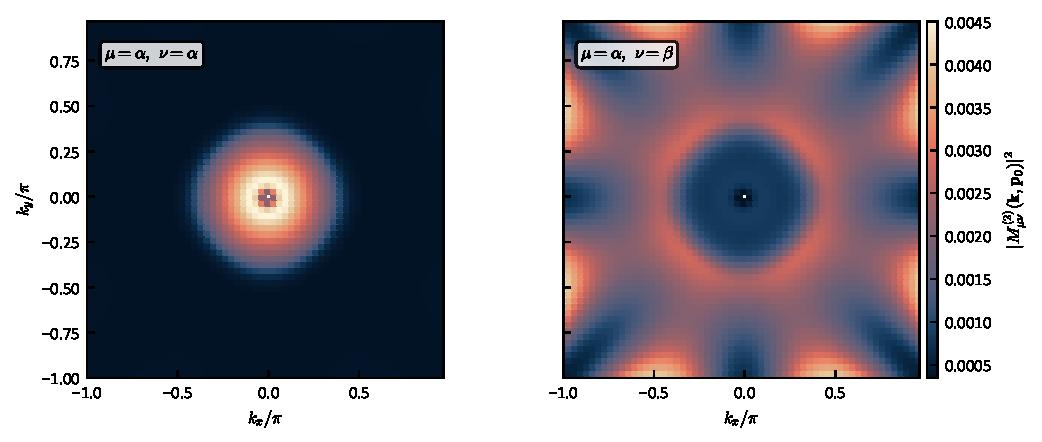
\includegraphics[width=1.0\textwidth]{figures/absM2_d=0.pdf}
    \centering
    \caption{Verteks pri $\vec d=0$ za $\vec{p}_0 =(0,0)$ za obe kopeli z disperzijo: $\omega_\vec{q}={\sqrt{\omega_0^2+c^2q^2}}$, $c=10, \omega_0=2.2$, indeks gor je indeks kopeli (za obe je tu enaka disperzija).}
\label{pic1}
\end{figure}
\begin{figure}[h!]
    \centering
    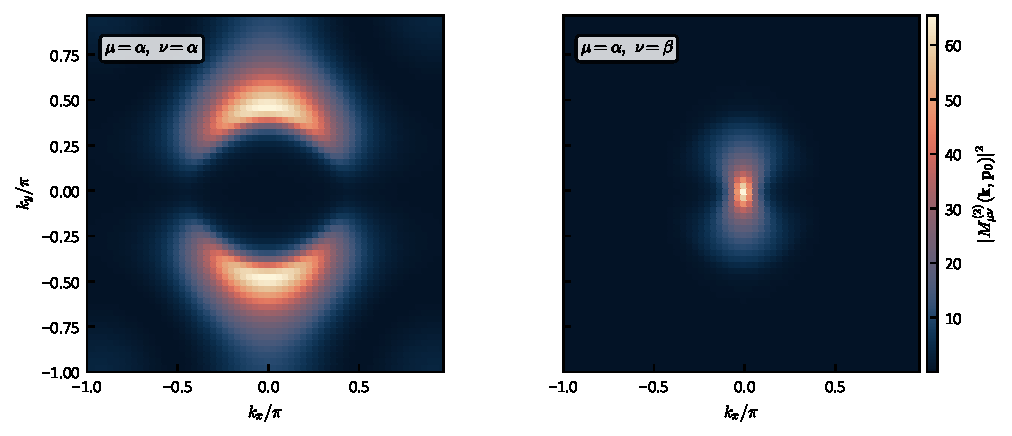
\includegraphics[width=1.0\textwidth]{figures/absM2_d=2.pdf}
    \centering
    \caption{Verteks pri $\vec d=(2, 0, 0)$ v $x$ smeri za $\vec{p}_0 =(0,0)$ za obe kopeli z disperzijo: $\omega_\vec{q}={\sqrt{\omega_0^2+c^2q^2}}$, $c=10, \omega_0=2.2$. Dipol zlomi $C_{4v} \to C_{2v}$ simetrijo.}
\label{pic1}
\end{figure}
\begin{figure}[h!]
    \centering
    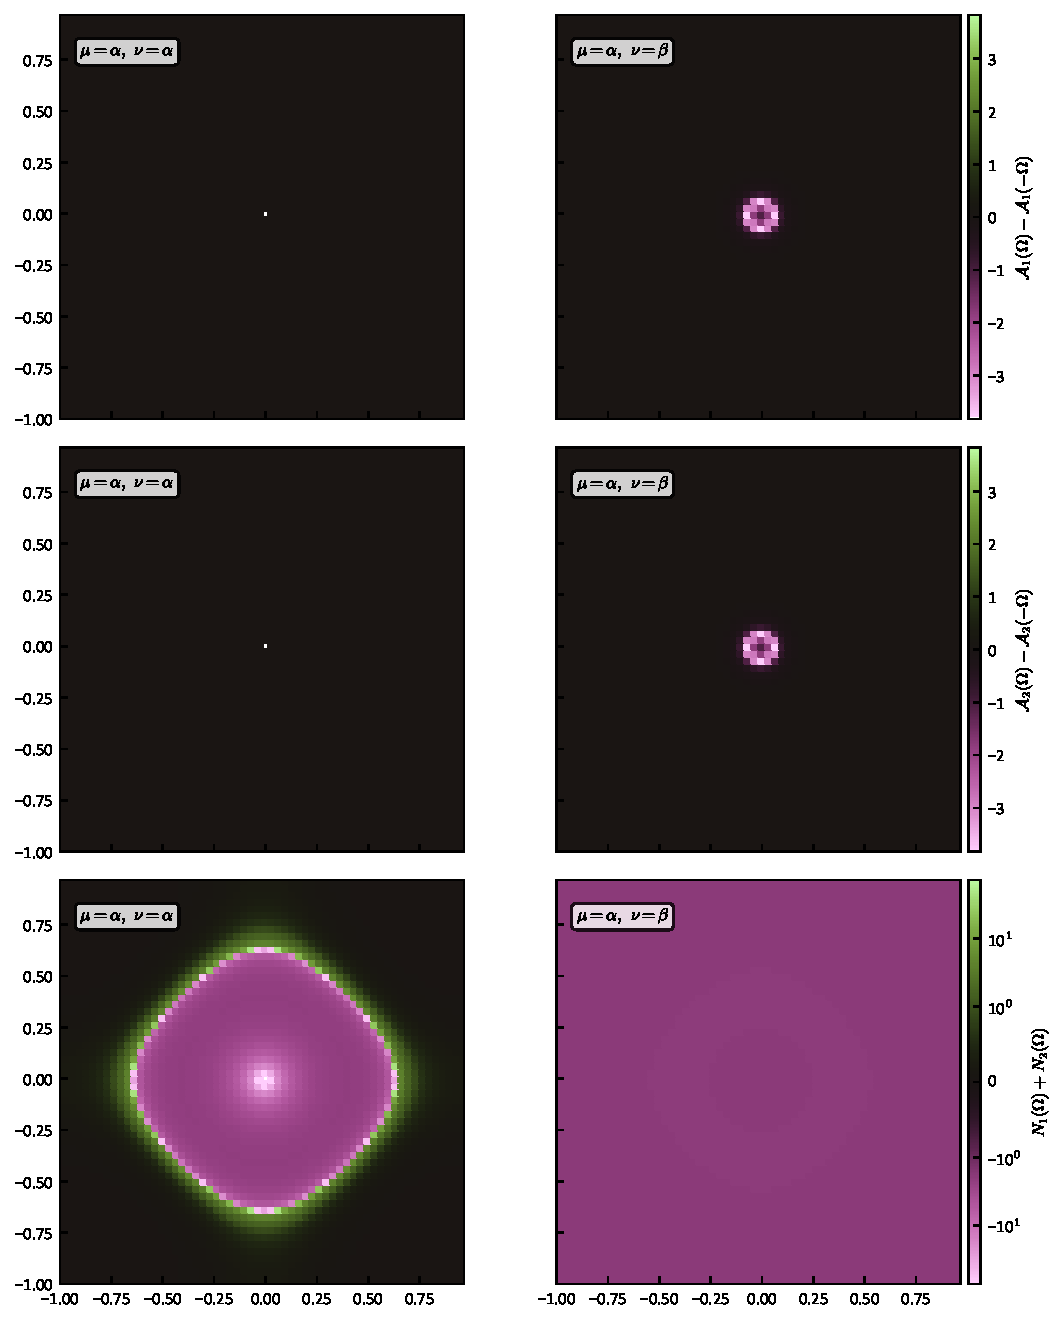
\includegraphics[width=1.0\textwidth]{figures/bath_components.pdf}
    \centering
    \caption{Komponente faktorjev za kopeli pri $\omega_\vec{q}={\sqrt{\omega_0^2+c^2q^2}}$, $c=10, \omega_0=2.2$ (majhni $q$ prehodi).}
\label{pic1}
\end{figure}
\begin{figure}[h!]
    \centering
    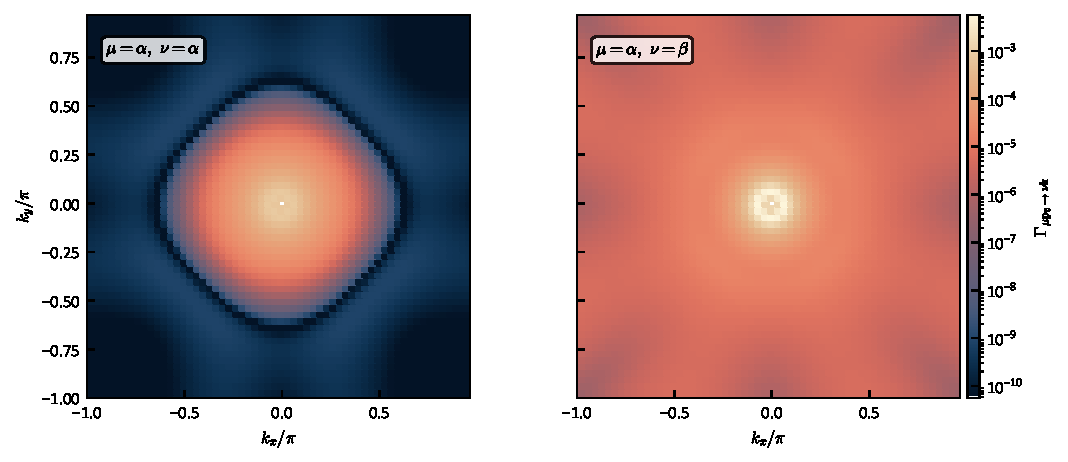
\includegraphics[width=1.0\textwidth]{figures/Gamma_d=0.pdf}
    \centering
    \caption{Končni transfer rate pri $\omega_\vec{q}={\sqrt{\omega_0^2+c^2q^2}}$, $c=10, \omega_0=2.2$, $\vec{d} = (0, 0, 0)$.}
\label{pic1}
\end{figure}
\begin{figure}[h!]
    \centering
    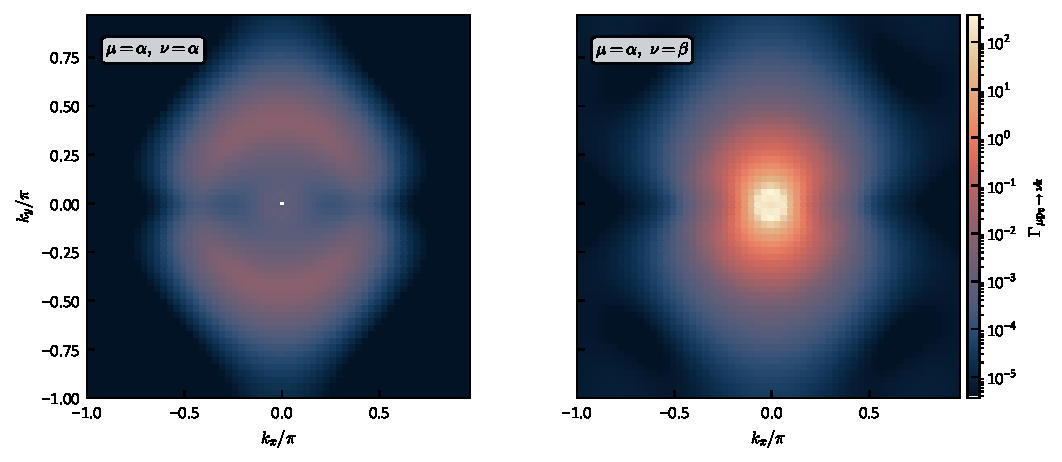
\includegraphics[width=1.0\textwidth]{figures/Gamma_d=2.pdf}
    \centering
    \caption{Končni transfer rate pri $\omega_\vec{q}={\sqrt{\omega_0^2+c^2q^2}}$, $c=10, \omega_0=2.2$, $\vec{d} = 2(1, 0, 0)$.}
\label{pic1}
\end{figure}
\begin{figure}[h!]
    \centering
    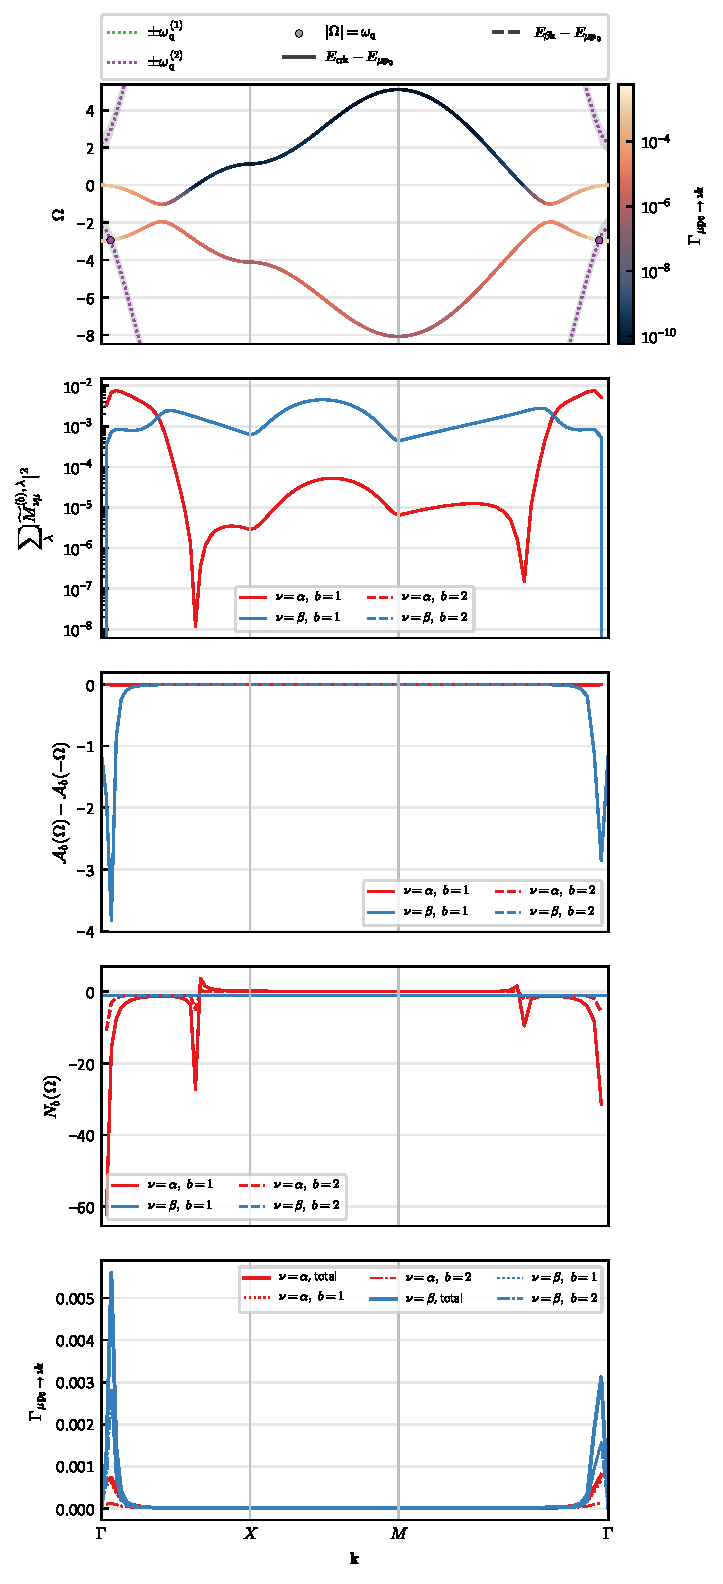
\includegraphics[width=0.49\textwidth]{figures/GamXM_path_bath_d=0.pdf}
    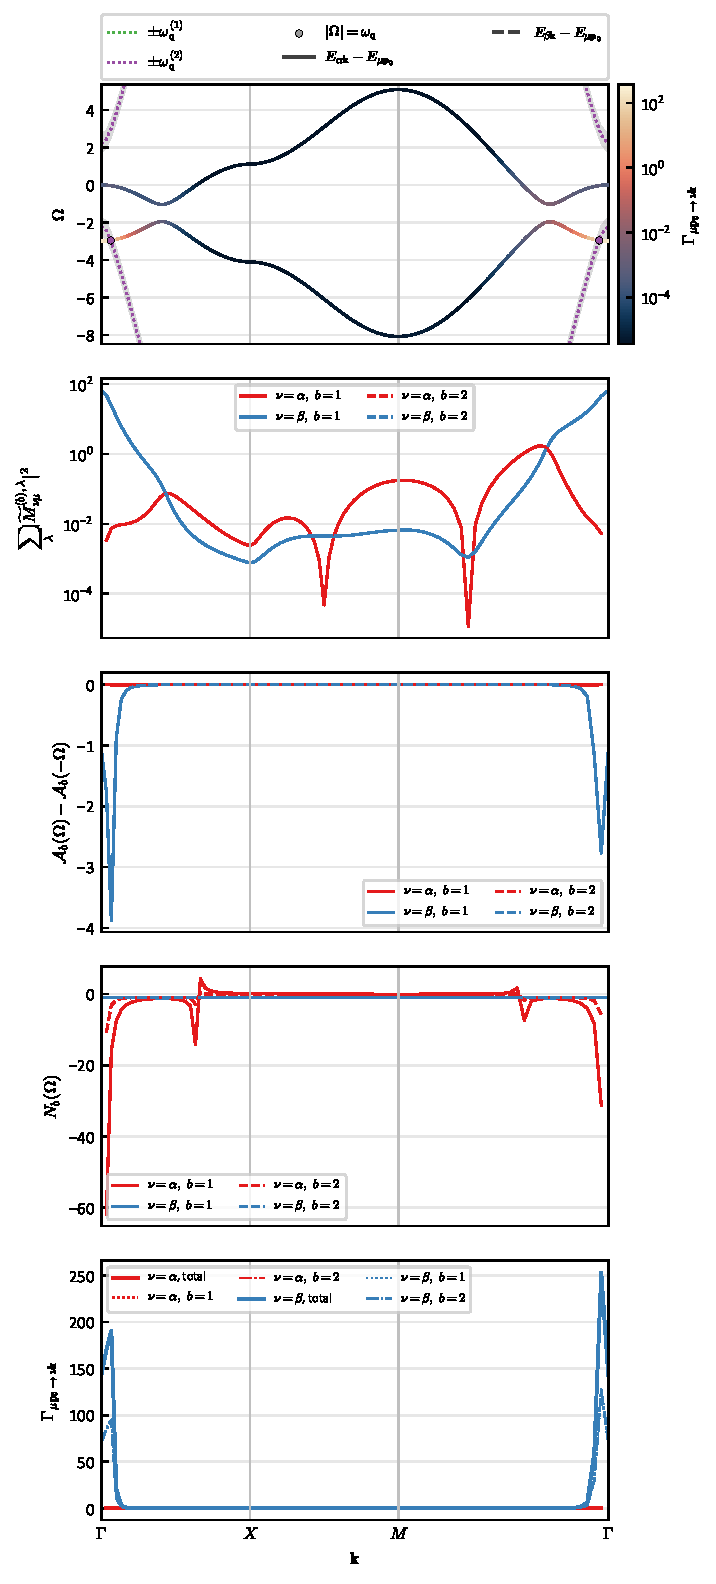
\includegraphics[width=0.49\textwidth]{figures/GamXM_path_bath_d=2.pdf}
    \centering
    \caption{Komponente faktorjev za kopeli pri $\omega_\vec{q}={\sqrt{\omega_0^2+c^2q^2}}$, $c=10, \omega_0=2.2$ (majhni $q$ prehodi).}
\label{pic1}
\end{figure}

\begin{figure}[h!]
    \centering
    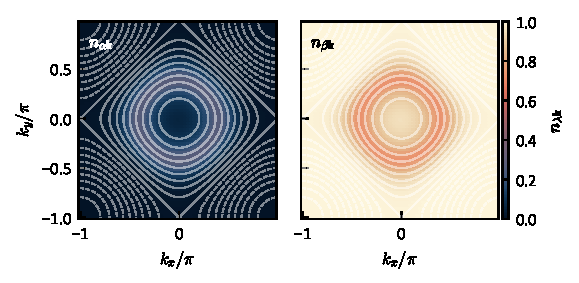
\includegraphics[width=0.49\textwidth]{figures/bz_d=0.pdf}
    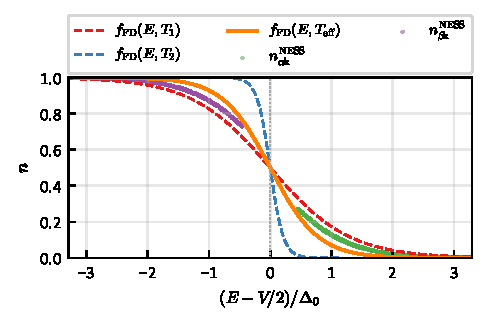
\includegraphics[width=0.49\textwidth]{figures/occ_E_d=0.pdf}
    \centering
    \caption{Komponente faktorjev za kopeli pri $\omega_\vec{q}={\sqrt{\omega_0^2+c^2q^2}}$, $c=10, \omega_0=2.2$ (majhni $q$ prehodi).}
\label{pic1}
\end{figure}



\begin{figure}[h!]
    \centering
    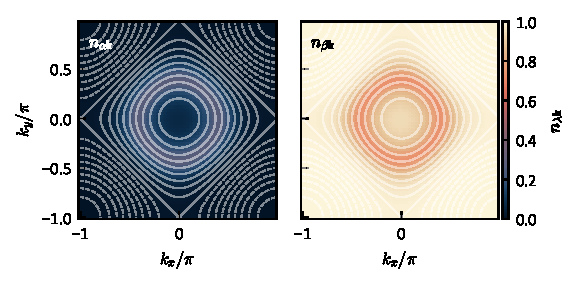
\includegraphics[width=0.49\textwidth]{figures/bz_d=2.pdf}
    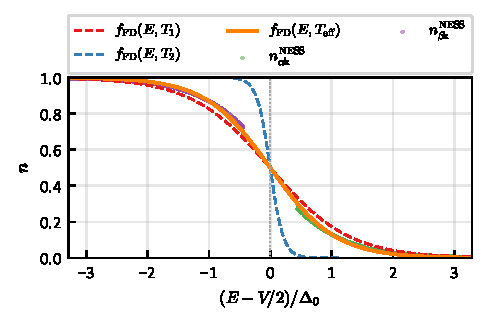
\includegraphics[width=0.49\textwidth]{figures/occ_E_d=2.pdf}
    \centering
    \caption{Komponente faktorjev za kopeli pri $\omega_\vec{q}={\sqrt{\omega_0^2+c^2q^2}}$, $c=10, \omega_0=2.2$ (majhni $q$ prehodi).}
\label{pic1}
\end{figure}
\begin{figure}[h!]
    \centering
    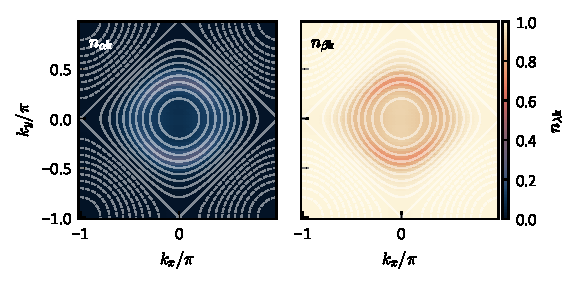
\includegraphics[width=0.49\textwidth]{figures/bz_d=0=1p6.pdf}
    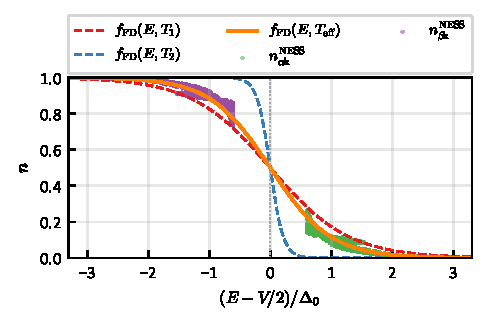
\includegraphics[width=0.49\textwidth]{figures/occ_E_d=0_c=1p6.pdf}
    \centering
    \caption{Komponente faktorjev za kopeli pri mixed disperzijah: $c=1.0$, $\omega_0^{(2)}=2.2$,  $\omega_0^{(1)}=0.1$ in  $\vec{d} = 2(1, 0, 0)$ zdaj zlomi simetrijo v $n(s)\to n(s, u)$, zgleda kar $C_{2v}$.}
\label{pic1}
\end{figure}
\begin{figure}[h!]
    \centering
    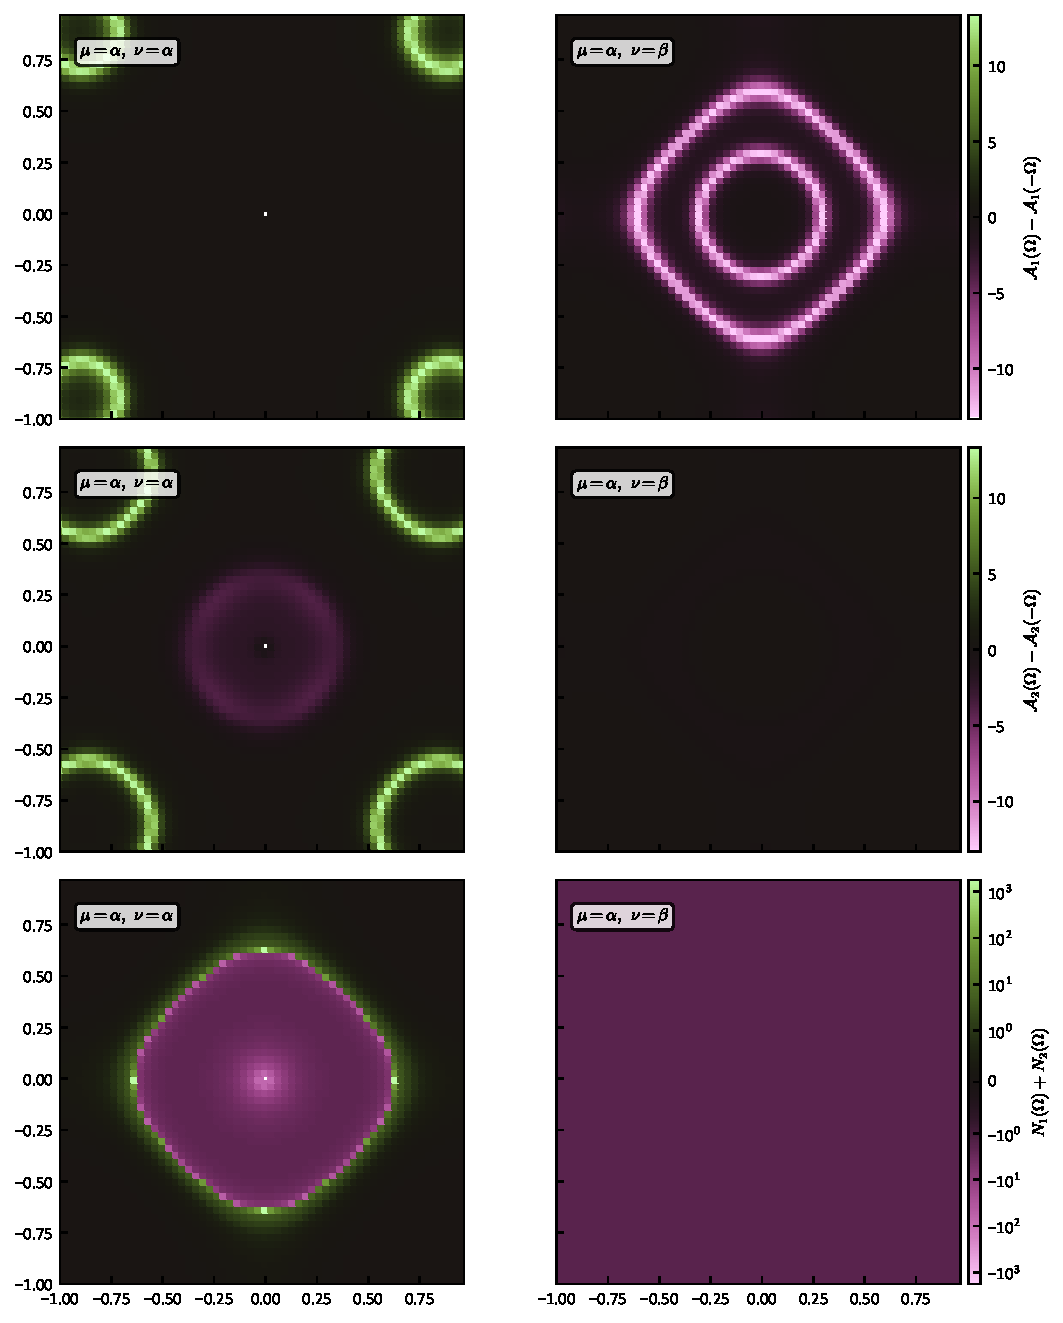
\includegraphics[width=1.0\textwidth]{figures/bath_components_mixed.pdf}
    \centering
    \caption{Komponente faktorjev za kopeli pri $c=1.0$, $\omega_0^{(1)}=2.2$,  $\omega_0^{(2)}=0.1$ in  $\vec{d} = 2(1, 0, 0)$ .}
\label{pic1}
\end{figure}

\begin{figure}[h!]
    \centering
    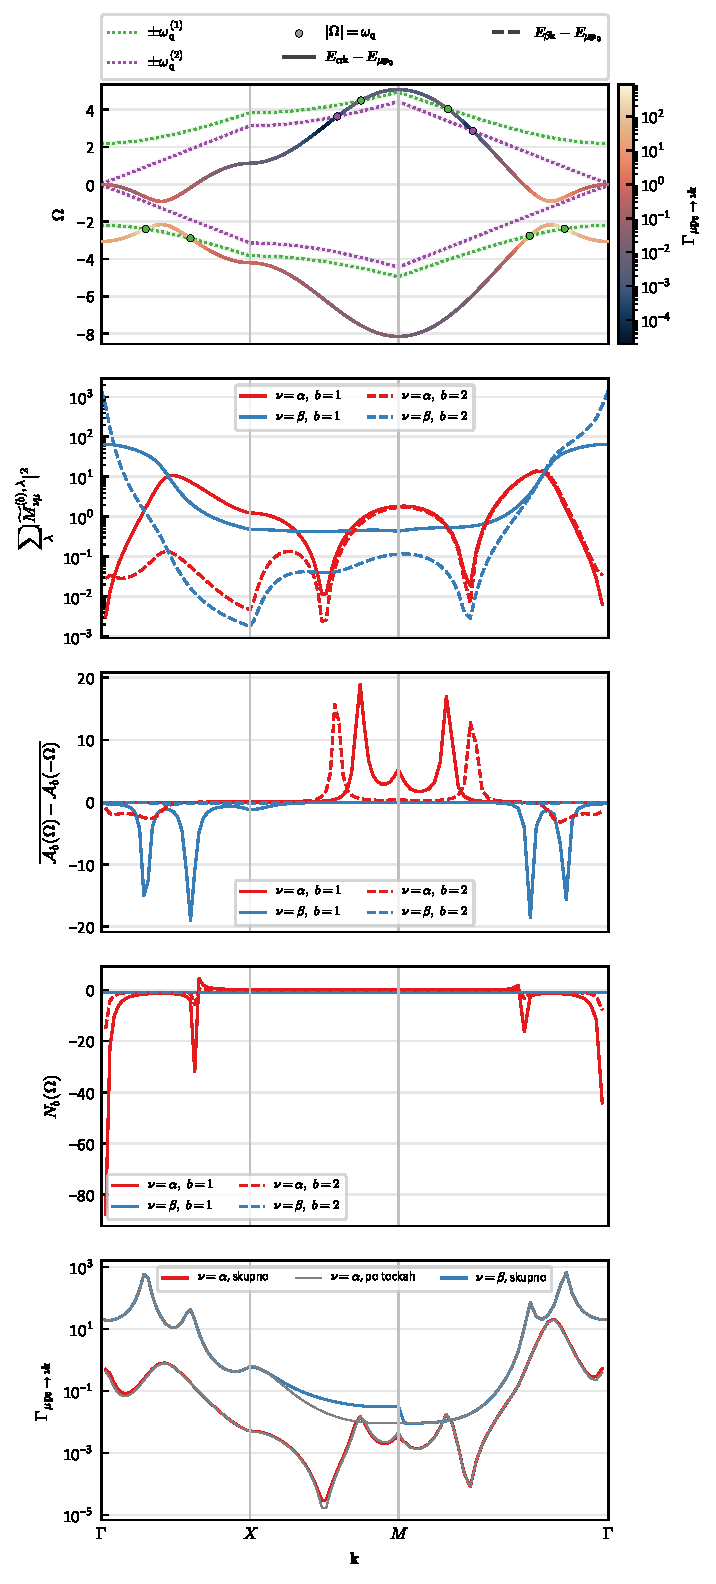
\includegraphics[width=0.65\textwidth]{figures/GamXM_path_bath_d=2_mixed.pdf}
    \centering
    \caption{Mixed disperzije: $c=1.0$, $\omega_0^{(1)}=2.2$,  $\omega_0^{(2)}=0.1$ in  $\vec{d} = 2(1, 0, 0)$.}
\label{pic1}
\end{figure}

\FloatBarrier

\subsection{Numerika detajli (konvergenca in povprecenje)}
Za manjše mreže nas zanima kaj se zgodi, če zgrešimo vrh resonance, ker je energija poračunana v neenakomerno razporejenih točkah. Zaradi tega lahko pogledamo, kaj se zgodi s povprečenjem čez sosednje točke. V 1D primeru je mreža definirana v točkah
\begin{gather}
k_i = i\,{\delta k},\qquad \mathcal C_i=\big[k_i-\tfrac{{\delta k}}{2},\,k_i+\tfrac{{\delta k}}{2}\big],\qquad
q_{ij}=k_i-k_j,\qquad \Omega_{ij}=E_{\nu}(k_i)-E_{\mu}(k_j),\\
\mathcal{S}(\Omega, \omega)=\mathcal{A}(\Omega)-{A}(-\Omega)
=\frac{8\gamma\,\omega\,\Omega}{\big[(\Omega-\omega)^2+\gamma^2\big]\big[(\Omega+\omega)^2+\gamma^2\big]}\,,
\qquad \omega_q=\sqrt{\omega_0^2+c_s^2q^2}\,.
\end{gather}
Po točkah bi računali:
\begin{equation}
\mathcal{S}^{\rm pt}_{ij}=\mathcal{S}\big(\Omega_{ij},\,\omega_{q_{ij}}\big).
\end{equation}
V svojih celicah sta $k$ in $p$ porazdeljena enakomerno, zato lahko napišemo povprečje čez celico kot
\begin{equation}
\overline{\mathcal{S}}_{ij}=\frac{1}{{\delta k}^{2}}\int_{\mathcal C_i}\,\dd{k}\int_{\mathcal C_j}\,\dd{p}\;
\mathcal{S}\big(E_\nu(k)-E_\mu(p),\,\omega_{k-p}\big)
=\int\! \dd{\Omega}\!\int\! \dd{q}\;\rho_{ij}(\Omega, q)\,\mathcal{S}(\Omega, \omega_q)\,,
\end{equation}
z vrjetnostno gostoto:
\begin{equation}
\rho_{ij}(\Omega, q)=\frac{1}{{\delta k}^{2}}\int_{\mathcal C_i}\!\,\dd{k}\int_{\mathcal C_j}\,\dd{p}\;
\delta\big(\Omega-E_\nu(k)+E_\mu(p)\big)\,\delta\big(q-k+p\big).
\end{equation}
 
% Energy binning: cell $i$ covers the energy interval
% \begin{equation}
% I_i=E_\nu(\mathcal C_i)=\Big[\min_{k\in\mathcal C_i}E_\nu,\ \max_{k\in\mathcal C_i}E_\nu\Big],
% \qquad |I_i|\simeq|E_\nu'(k_i)|\,{\delta k} ,
% \end{equation}
% so $\Omega$ spreads over $I_i-I_j$, of width $\simeq\big(|E_\nu'(k_i)|+|E_\mu'(k_j)|\big){\delta k}$.
Naredil sem približek, kjer razlike energij odčitamo točno v diskretnih točkah, povprečimo pa čez momente (skupna verjentostna gostota za razliko dveh enakomernih spremeljivk $q = k-p$ je konvolucija, torej trikotna funkcija $P$)
\begin{equation}
\rho_{ij}(\Omega, q)\;\approx\;\delta(\Omega-\Omega_{ij})\,P(q-q_{ij}),\qquad
P(x)=\frac{1}{{\delta k}}\Big(1-\frac{|x|}{{\delta k}}\Big)\,\Theta({\delta k}-|x|),\qquad \int P=1\,,
\end{equation}
kar nam da skupaj pri fiksni energijski razliki $\Omega_{ij} = E_\nu(k_i)-E_\mu(p_j)$:
\begin{equation}
{\;\overline{\mathcal{S}}_{ij}\approx\int_{q_{ij}-{\delta k}}^{\,q_{ij}+{\delta k}}\!dq\;P(q-q_{ij})\,\mathcal{S}(\Omega_{ij}, \omega_q)\;}
\end{equation}
V praksi to pomeni, da vzamemo $n_s$ točk in seštejemo namest integriramo: 
\begin{equation}
t_l=2\Big[\frac{l-\frac12}{n_s}-\frac12\Big],\qquad
,\qquad \sum_{l=1}^{n_s}\frac{2}{n_s}\big(1-|t_l|\big)=1,
\qquad l=1,\dots,n_s ,
\end{equation}
oz. diskretno (z upeljavo $t = (q-q_{ij})/\delta k$) za arbitrarno funkcijo $F(q)$:
\begin{equation}
\int_{-1}^{1}\,\dd{t}\,(1-|t|)\,F(q_{ij} + t\delta k)=\sum_l\frac{2}{n_s}\big(1-|t_l|\big)  F(q_{ij} + t_l \delta k)+\mathcal O(n_s^{-2}).
\end{equation}
V principu se lahko tu ustavimo, ampak je računanje za vsak par $\Omega_{ij}$ zahtevno $\mathcal{O}((2 N_k^2)^2 n_s^2)$ (veliko parov $\vec q_{ij}$ da enako energijo, ker je $\Omega = \Omega(s)$). Zato tabeliramo razlike energij in interpoliramo. Izbral sem $\delta \Omega = \gamma / 8$, tako je $N_\Omega = \lceil{E_\text{max} / \delta \Omega\rceil} + 2$, kjer si $E_\text{max}$ izberemo tako, da je večji od največje možne razlike energij\footnote{V kodi to oceim avtomatsko navzgor z 10\% maržo.}. Za neko funkcijo $F(\Omega)$ potem računamo le $N_\Omega$ točk in za določen $\Omega_n\leq \Omega_{ij}\leq \Omega_{n+1}$ interpoliramo linearno: 
\begin{align}
  F(\Omega) = (1-\alpha)F(\Omega_n) + \alpha F(\Omega_{n+1})\,,\quad \alpha = \Omega/\delta\Omega - \lfloor\Omega/\delta\Omega\rfloor
\end{align}
to skupaj stane $N_k^2 N_\Omega n_s^2 + (2N_k)^2$, dodatni clen je za lookup. Na koncu se bolj splača skupaj povprečiti ne le spektralno funckijo, temvec tudi dodatne faktorje. S krajšo notacijo:  
\begin{align}
  \vec h=\Big(\sin\big(k'_x+\tfrac{q_x}{2}\big),\ \sin\big(k'_y+\tfrac{q_y}{2}\big)\Big)
\end{align}
in
\begin{align}
  Z_{xx}=\sin^2\!\varphi+(\omega_0/\omega_{\vec q})^2\cos^2\!\varphi,\qquad Z_{yy}=\cos^2\!\varphi+(\omega_0/\omega_{\vec q})^2\sin^2\!\varphi,\qquad Z_{xy}=2\sin\varphi\cos\varphi\,((\omega_0/\omega_{\vec q})^2-1),
\end{align}
definiramo še (bolj stabilno v kodi, tudi produkt $\Omega N(\Omega)$ je stabilen za $\Omega \to 0$):
\begin{align}
  F_\vec{q}(\Omega)=\frac{\mathcal{A}_{\vec q}(\Omega)-\mathcal{A}_{\vec q}(-\Omega)}{\Omega\omega_{\vec q}}= \frac{8\gamma}{\big[(\Omega-\omega)^2+\gamma^2\big]\big[(\Omega+\omega)^2+\gamma^2\big]}\,,
\end{align}
tako je po točkah (to je enaka matrika kot \eqref{gam_photon_numerika})
\begin{align}
  \Gamma_{\gamma'\vec{k}'\to\gamma \vec{k}}=A \cdot \Omega N(\Omega) \cdot \Big[\big(h_x^2Z_{xx}F_{\vec q}+h_y^2Z_{yy}F_{\vec q}+h_xh_yZ_{xy}F_{\vec q}\big)C_{\gamma\gamma'}^2+Z_{xx}F_{\vec q}D_{\gamma\gamma'}^2\Big]\,,
\end{align}
Povprečimo produkte tipa $Z_{xx}F_{\vec q}$ s trikotno funkcijo, medtem ko $\vec h$, $C_{\gamma, \gamma'}$ in $\Omega$ računamo le v centrih celic: 
\begin{tcolorbox}
\begin{align}
  \overline\Gamma_{\gamma'\vec k'\to\gamma \vec k}=A \cdot \Omega N(\Omega)\cdot  \Big[\left(h_x^2 \overline{Z_{xx}F_{\vec q}}+h_y^2 \overline{Z_{yy}F_{\vec q}}+h_xh_y \overline{Z_{xy}F_{\vec q}}\right)C_{\gamma\gamma'}^2+ \overline{Z_{xx}F_{\vec q}} D_{\gamma\gamma'}^2\Big]\,,
\end{align}
\end{tcolorbox} \noindent
kjer je 
\begin{align}
  \overline{X_{\vec{q}}(\Omega)} =\int\,\dd{x}\dd{y}P(x)P(y)\,X_{(q_x + x, q_y + y)}\;\simeq\sum_{l,m}^{n_s}\left( \frac{2}{n_s}\right)^2\big(1-|t_l|\big)\big(1-|t_m|\big)X_{\vec{q}+(t_l\delta k_x,\,t_m\delta k_y)}\,.
\end{align}


\begin{figure}[h!]
    \centering
    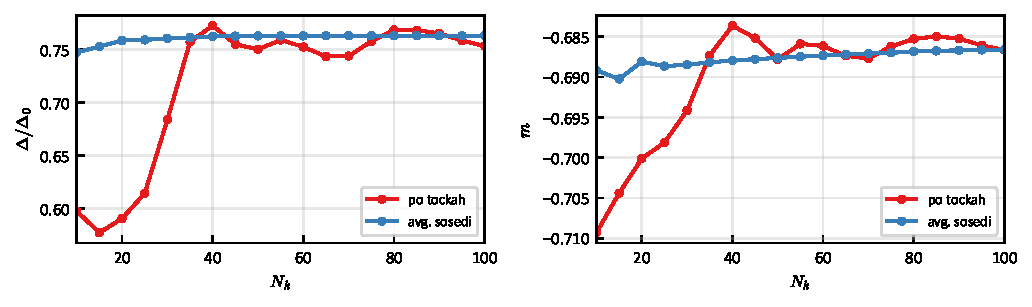
\includegraphics[width=1\textwidth]{figures/N_k_convergence.pdf}
    \centering
    \caption{Mixed disperzije: $c=10.0$, $\omega_0^{(1)}=2.2$,  $\omega_0^{(2)}=0.1$ in  $\vec{d} = 2(1, 0, 0)$ ter $\gamma=0.1$. KOnvergenca pri $T_1 = 1.2T_c$ in $T_2 = 0.2T_c$. TO je za primer ko je $q\ll k_F$, tako da so small momentum prehodi, vecinoma interband (diagonalna baza).}
\label{pic1}
\end{figure}

\begin{figure}[h!]
    \centering
    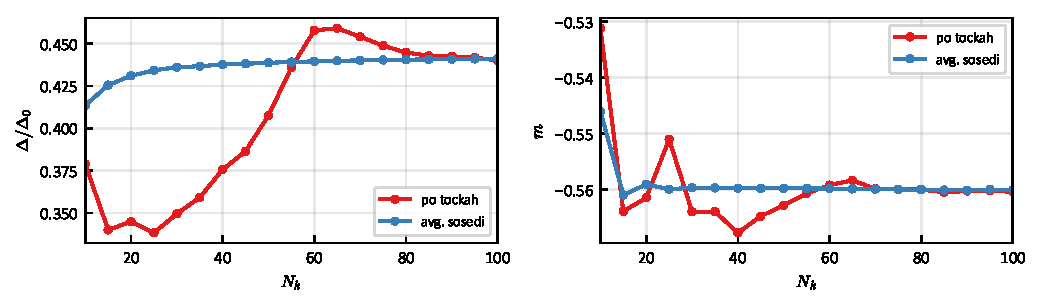
\includegraphics[width=1\textwidth]{figures/N_k_convergence2.pdf}
    \centering
    \caption{Mixed disperzije: $c=10.0$, $\omega_0^{(1)}=2.2$,  $\omega_0^{(2)}=0.1$ in  $\vec{d} = 2(1, 0, 0)$ ter $\gamma=0.1$. KOnvergenca pri $T_1 = 2.5T_c$ in $T_2 = 0.2T_c$. TO je za primer ko je $q\ll k_F$, tako da so small momentum prehodi, vecinoma interband (diagonalna baza) (dlje od diagonale $T_1=T_2$ pocasneje konvergira).}
\label{pic1}
\end{figure}

\begin{figure}[h!]
    \centering
    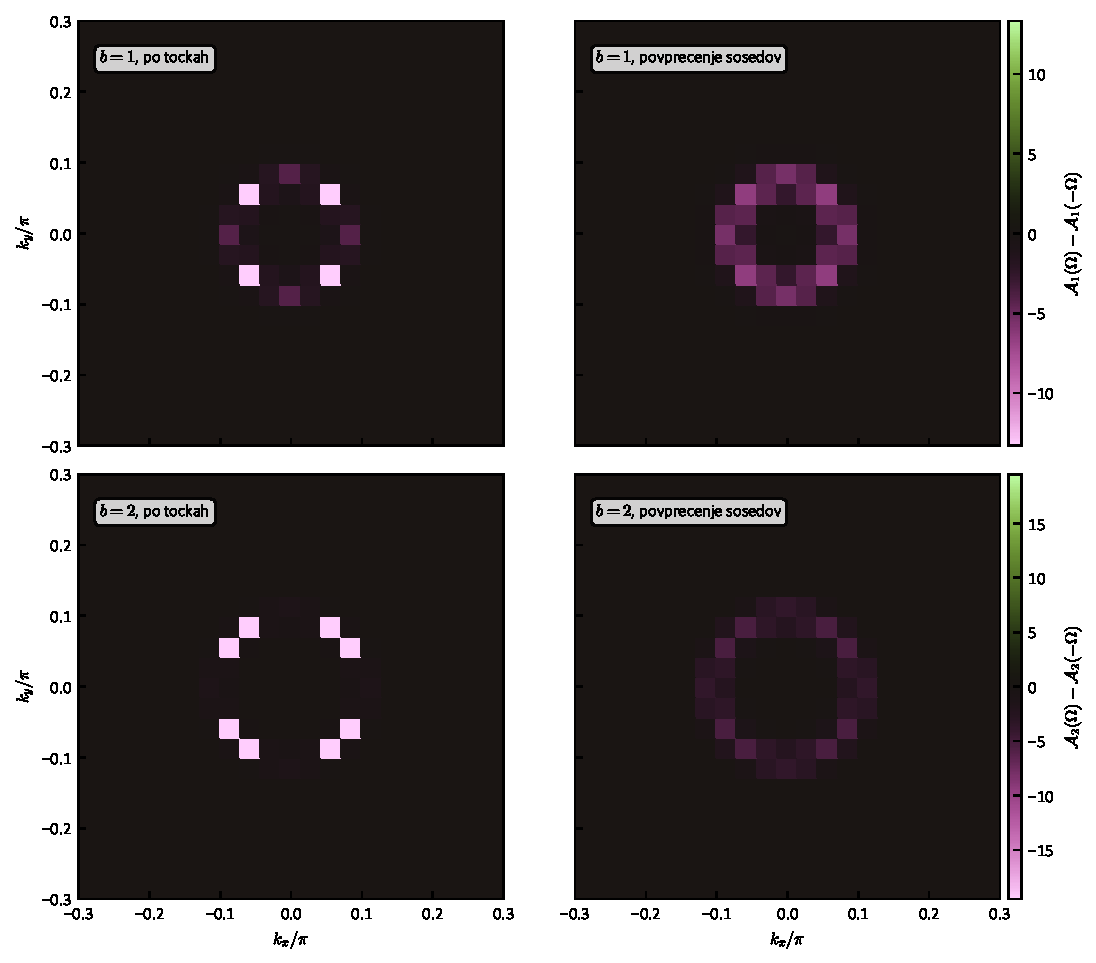
\includegraphics[width=1\textwidth]{figures/primerjava_potockah_lorentz_grid.pdf}
    \centering
    \caption{.}
\end{figure}

\begin{figure}[h!]
    \centering
    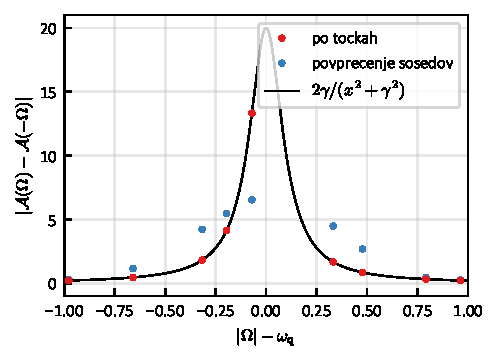
\includegraphics[width=0.49\textwidth]{figures/primerjava_potockah_lorentz.pdf}
    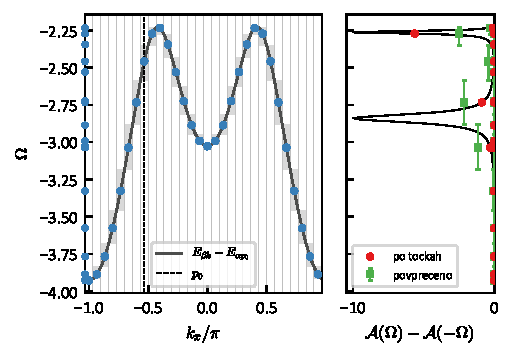
\includegraphics[width=0.49\textwidth]{figures/cut_line_01.pdf}
    \centering
    \caption{.}
\end{figure}

\subsubsection{Andersonov algoritem}
Samokonsistenten sistem enačb je ekvivalenten reševanju fixed point problema $\vec{x} = \mathcal{G}(\vec{x})$, oziroma iskanje ničel funckije $\vec f(\vec x)=\mathcal G(\vec x)-\vec x$. Pri Picard iteracijah samo posodabljamo s prejšnjo vrednostjo:
\begin{align}
  \vec x_{k+1}=\vec x_k+\beta\,\vec f_k \,.
\end{align}

okoli rešitve se konvergenca ustavi, saj je: $\vec f(\vec x)\approx J(\vec x-\vec x^*)$ kjer je Jakobijan $J=\partial\mathcal G/\partial\vec x-
\mathds{1}$. 
\begin{figure}[h!]
    \centering
    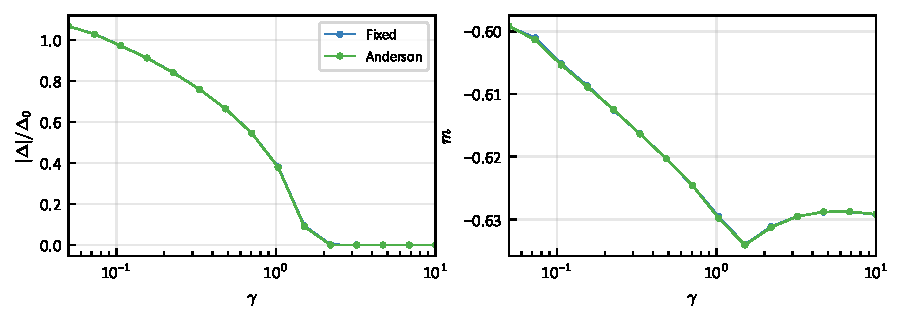
\includegraphics[width=1.\textwidth]{figures/gamma_D_m_sweep.pdf}
    \centering
    \caption{$G=2, t_a=-t_b=1$ in $V=7.8$, kjer je $\Delta_0=1.0$. Disperziji sta: $c=10.0$, $\omega_0^{(1)}=3.0$,  $\omega_0^{(2)}=0.01$. V sklopitvi je $d = 2$ in $N_k=65$, $n_s = 8$. V točki $T_1 = 4.4 T_c$ in $T_2 =0.01T_c$.}
\end{figure}
\begin{figure}[h!]
    \centering
    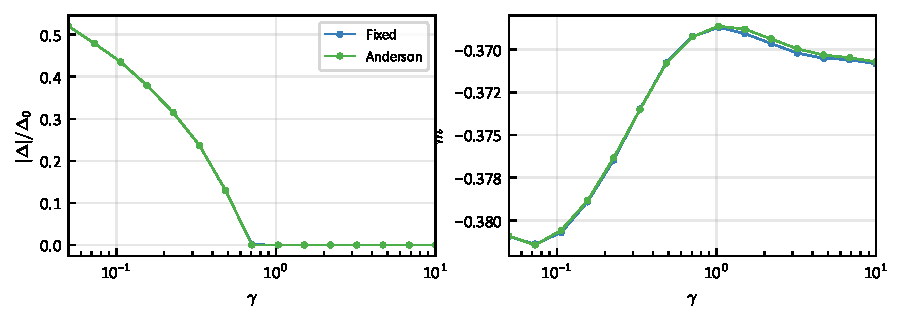
\includegraphics[width=1.\textwidth]{figures/gamma_D_m_sweep_BCS.pdf}
    \centering
    \caption{$G=2, t_a=-t_b=1$ in $V=4.4$, kjer je $\Delta_0=1.0$. Disperziji sta: $c=10.0$, $\omega_0^{(1)}=3.0$,  $\omega_0^{(2)}=0.01$. V sklopitvi je $d = 2$ in $N_k=65$, $n_s = 8$. V točki $T_1 = 4.4 T_c$ in $T_2 =0.01T_c$.}
\end{figure}
\FloatBarrier
\subsection{Primer NESS za BEC}
Primer NESS v BEC režimu: $G=2, t_a=-t_b=1$ in $V=7.8$, kjer je $\Delta_0=1.0$. Disperziji sta: $c=10.0$, $\omega_0^{(1)}=2.2$,  $\omega_0^{(2)}=0.01$. V sklopitvi je $d = 2$ in $\gamma=0.15$ in $N_k=50$. 
\begin{figure}[h!]
    \centering
    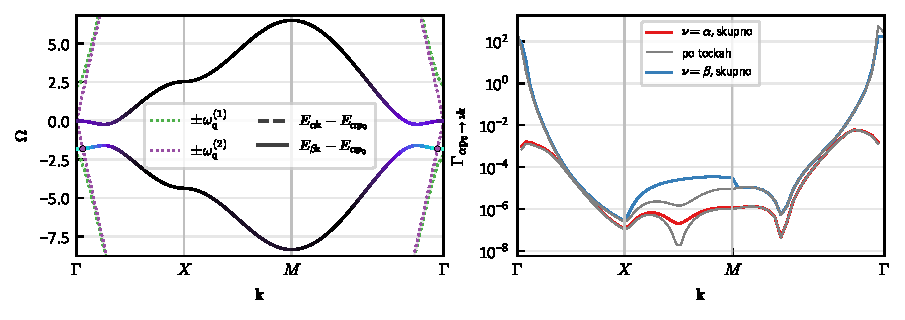
\includegraphics[width=1\textwidth]{figures/GamXM_path_bath_BEC_primer.pdf}
    \centering
    \caption{Grafi so v točki $T_1 = 4.4 T_c$ in $T_2=0.01T_c$, kjer preidemo v BCS režim.}
\end{figure}
\begin{figure}[h!]
    \centering
    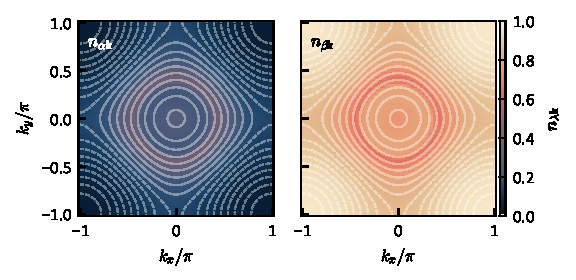
\includegraphics[width=0.49\textwidth]{figures/bz_occ_BEC_primer.pdf}
    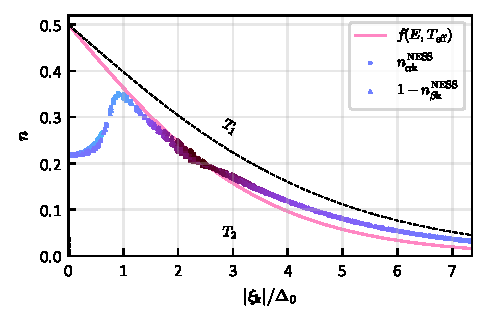
\includegraphics[width=0.49\textwidth]{figures/xi_occ_BEC_primer.pdf}
    \centering
    \caption{Grafi so v točki $T_1 = 4.4 T_c$ in $T_2=0.01T_c$, kjer preidemo v BCS režim.}
\end{figure}
\begin{figure}[h!]
    \centering
    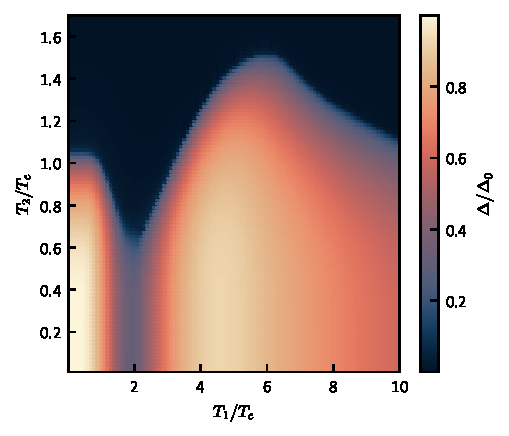
\includegraphics[width=0.49\textwidth]{figures/gap_map_BEC_test.pdf}
    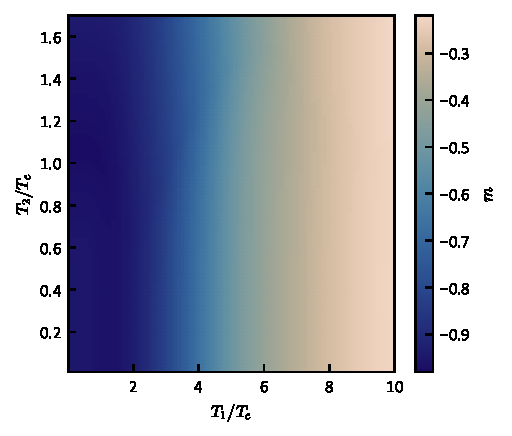
\includegraphics[width=0.49\textwidth]{figures/m_map_BEC_test.pdf}
    \centering
    \caption{Disperziji sta: $c=10.0$, $\omega_0^{(1)}=3$,  $\omega_0^{(2)}=0.01$, BEC režim.}
\end{figure}
\begin{figure}[h!]
    \centering
    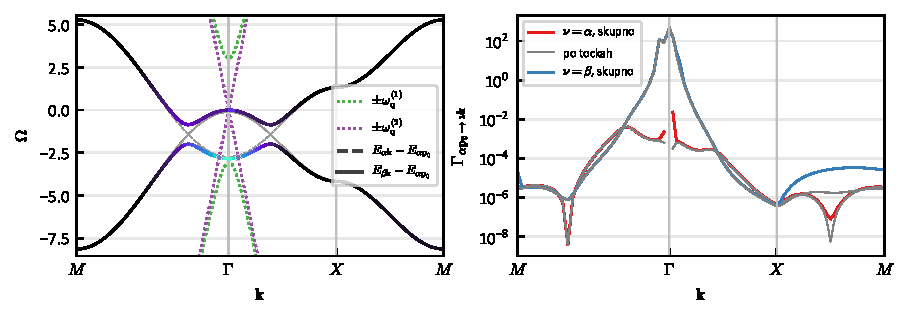
\includegraphics[width=1\textwidth]{figures/GamXM_path_BEC_nadTc.pdf}
    \centering
    \caption{Disperziji sta: $c=10.0$, $\omega_0^{(1)}=3$,  $\omega_0^{(2)}=0.01$. Grafi so v točki $T_1 = 6.0 T_c$ in $T_2=1.3T_c$, kjer preidemo v BCS režim.}
\end{figure}
\begin{figure}[h!]
    \centering
    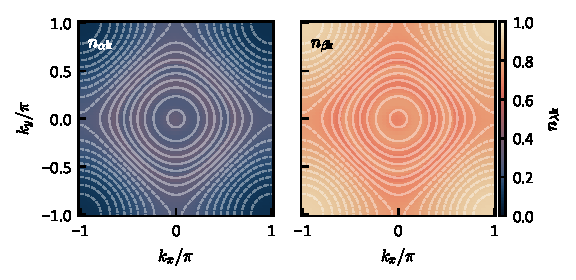
\includegraphics[width=0.49\textwidth]{figures/bz_BEC_nadTC.pdf}
    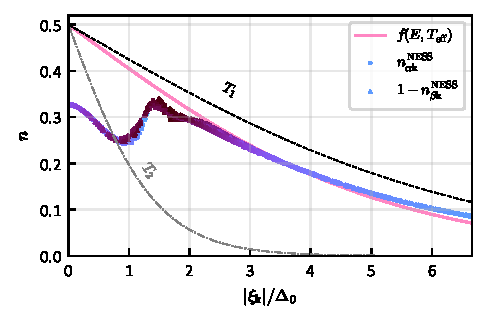
\includegraphics[width=0.49\textwidth]{figures/occ_xi_BEC_nadTC.pdf}
    \centering
    \caption{Disperziji sta: $c=10.0$, $\omega_0^{(1)}=3$,  $\omega_0^{(2)}=0.01$. Grafi so v točki $T_1 = 6.0 T_c$ in $T_2=1.3T_c$, kjer preidemo v BCS režim.}
\end{figure}
\FloatBarrier

\subsection{Primer NESS za BCS}
Primer NESS v BCS režimu: $G=2, t_a=-t_b=1$ in $V=4.4$, kjer je $\Delta_0=1.0$. Disperziji sta: $c=10.0$, $\omega_0^{(1)}=3.0$,  $\omega_0^{(2)}=0.01$. V sklopitvi je $d = 2$ in $\gamma=0.15$ in $N_k=50$. 
\begin{figure}[h!]
    \centering
    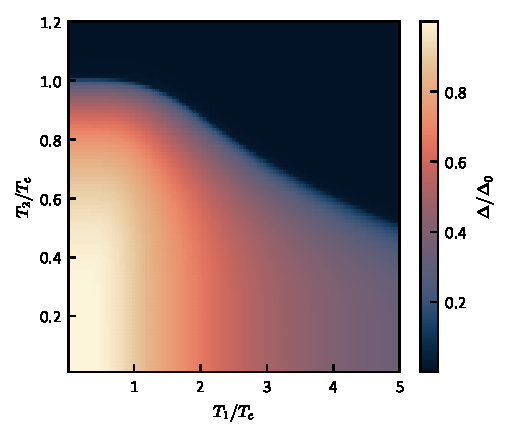
\includegraphics[width=0.49\textwidth]{figures/gap_map_BCS_test.pdf}
    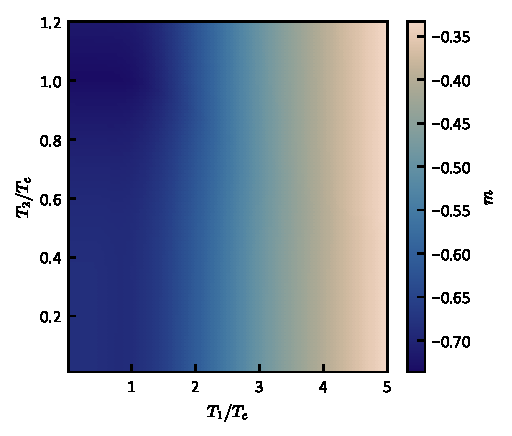
\includegraphics[width=0.49\textwidth]{figures/m_map_BCS_test.pdf}
    \centering
    \caption{Disperziji sta: $c=10.0$, $\omega_0^{(1)}=3$,  $\omega_0^{(2)}=0.01$, BEC režim.}
\end{figure}
\FloatBarrier

\nocite{*}
\printbibliography
\end{document} 